\chapter{Modified Quadratic Estimator}
\label{ch:mqe}
\section*{Overview}\label{ovr}
In the last chapter ~\ref{tSZ_effect_bias} we saw that the thermal Sunayev-Zel'dovich (referred as SZ hereafter) effect is a major contamination in the CMB-cluster lensing analysis. 
One of the ways to mitigate the SZ induced systematic bias in the Maximum Likelihood Estimator (MLE) is by using SZ-free maps.
However, SZ-free maps have higher noise resulting in decrease of signal to noise ratio (SNR) by a factor of three. 
%However, that would result in a decrease of signal to noise ratio (SNR) by a factor of three due to the higher noise level of tSZ-free maps. 
%On the other hand, the Quadratic Estimator can be modified to eliminate the SZ systematic bias with only a slight decrease of SNR.
 During my thesis, we developed a modified Quadratic Estimator (mQE) to eliminate the bias due thermal Sunyaev Zel'dovich (SZ) effect with only a slight decrease in SNR. 


This chapter is organised as follows. First, we provide a brief review of the SZ effect in ~\ref{SZ} (refer \cite{sunyaev70b} for a detailed review) and its effect on CMB-cluster lensing in \S\ref{sec_sz_induced_bias}.
We discuss the modifications done to the QE in order to remove the SZ bias in \S\ref{sec_method}.
 %We explain the data sets used in \S\ref{sec_data} and the model fitting in \S\ref{sec_model_fitting}. 
 The datasets and model fitting are described in  \S\ref{sec_model_fitting} and \S\ref{sec_data} respectively.
 Before we apply our new method to data in \S\ref{mqe_sec_results}, we validate our pipeline using simulations in \S\ref{sec:pipeline_verfication}. The effect of systematics involved in the analysis  is quantified in \S\ref{mqe_sec_systematics}.
Finally, we conclude in \S\ref{sec_con}. %we compare our results with similar work in \S\ref{mqe_sec_results}.
This chapter closely follows \citet{raghunathan18}.%\citet*{raghunathan18_2}
%We explain the constraints on mass-richness scaling relation obtained using the above data. 


\section{Thermal Sunayev-Zel'dovich effect}\label{SZ}

 The Cosmic microwave background (CMB) photons get inverse Thompson scattered off the high energy electrons present in the intra cluster medium of a galaxy cluster, resulting in the deficiency of photons at lower frequencies and excess of photons at higher frequencies. 
 This phenomena is called the thermal Sunayev-Zel'dovich (SZ) effect. 
 The SZ is a small effect and we illustrate it by showing the CMB spectral distortion for a fictional galaxy cluster 1000 times more massive than a typical galaxy cluster in Fig. ~\ref{ned_plot}. %to illustrate it we have shown the CMB spectral distortion for a fictional galaxy cluster 1000 times more massive than a typical galaxy cluster in Fig. ~\ref{ned_plot}. % check_again
 The solid black curve represents the intensity of the CMB as a function of frequency before its interaction with hot intracluster medium and the solid blue represents the same after its interaction.
 As shown in the Fig.~\ref{ned_plot}, due to the SZ effect CMB intensity decreases below a frequency of $\sim$220 \,GHz and increases at higher frequencies. 
   
The fractional change in temperature is given by 
\begin{equation}
\label{eq:sz_eqn}
\frac{\Delta T_{SZ}}{T_{CMB}} = f(x) y = f(x) \int n_{e} \frac{k_{B}T_{e}}{m_{e}c^{2}} \sigma_{T} dl
\end{equation}
where $y$ is Compton $y$-parameter, $n_{e}$ is the electron number density, $m_{e}$ is the electron rest mass, $c$ is the speed of light,  $T_{e}$ is the electron temperature, $\sigma_{T}$ is the Thompson cross-section, and $f(x)$ is the dimensionless frequency given by
\begin{equation}
f(x) = \left(x\frac{e^{x}+1}{e^{x}-1} -4 \right ) \left(1 + \delta_{SZE}(x,T_{e}) \right)
\end{equation} 
where $\delta_{SZE}(x,T_{e})$ is the relativistic correction to the frequency dependence.
\begin{figure}[ht]
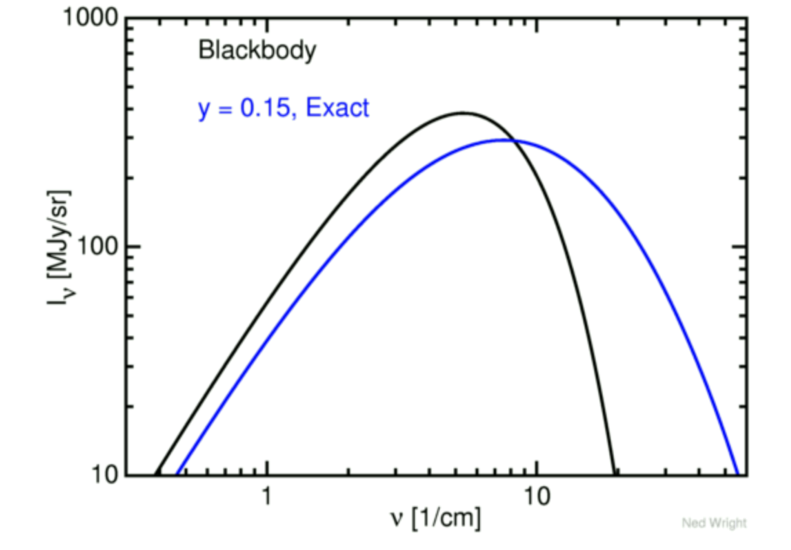
\includegraphics[width=\linewidth]{figs/tSZ_effect_Ned.png}
\caption{The plot shows the intensity of CMB as function of frequency before (black) and after (blue) it passes through a cluster. Credits: {Ned Wright, UCLA} }
\label{ned_plot}
\end{figure}

The CMB surveys make use of the SZ effect to detect galaxy clusters which appear as a semi-resolved negative signal decrement at frequencies lower than 220 GHz.
As can be inferred from Eq. \ref{eq:sz_eqn}, the SZ effect is independent of redshift and has the potential to detect high redshift clusters, where the cluster abundance critically depends on the underlying cosmological model.
%The CMB surveys make use the SZ effect to detect galaxy clusters which appear as a blue blob at frequencies lesser than 220 GHz.

Fig. \ref{fig:clus_in_cmb} shows a galaxy cluster of mass $M_{200m}= 5 \times 10^{14} M_{\odot}$\footnote{$M_{200m}$ is defined as the mass of the cluster within radius, $R_{200}$, within which the cluster density is 200 times the mean density of the Universe at cluster redshift.}  at a redshift of $z = 0.7$ as observed by a CMB survey in 90 GHz and 150 GHz channels. While the beam size of 90 GHz channel is bigger than the 150 GHz for a given CMB experiment, here we have assumed the beam sizes of both frequency channels to be 1\am\ in order to show the amplitude difference.  
\begin{figure}[ht]
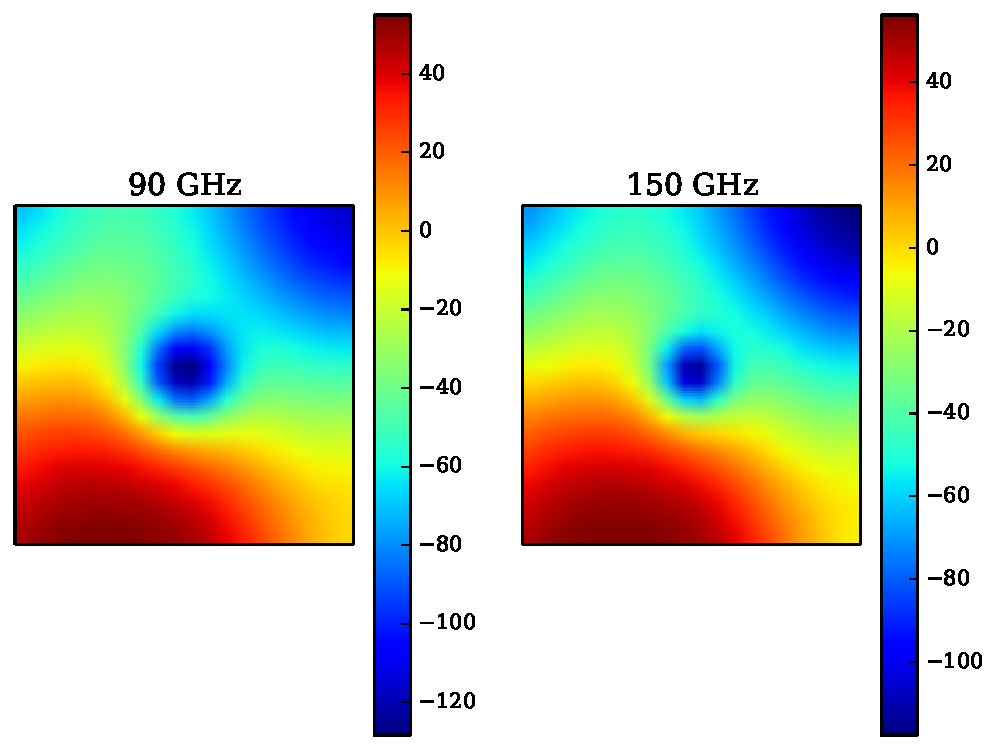
\includegraphics[width=\linewidth]{figs/clus_in_cmb_new}
\caption{A galaxy cluster of mass $M_{200m} = 5 \times 10^{14} M_{\odot}$ at redshift of $z = 0.7$ as observed by a CMB survey with a beam size of 1\am\ in both 90 and 150 GHz channels.  % \footnote{in general beam size of 90 \,GHz channel is bigger than \,150 GHz}
 Each image extends \smallboxsize \; and the colorbar is $\mu$K. It is worth noting that the amplitude of SZ signal in the 90 GHz channel is higher by a factor $\sim$ 1.67 compared to the corresponding SZ signal in the 150 GHz channel.}
\label{fig:clus_in_cmb}
\end{figure}
 %Effect of SZ signal on CMB lensing is discussed in ~\ref{sec_sz_induced_bias}.
 
 



%\section{Methods}
%This section is organised as follows: quadratic estimator is explained in \S\ref{qe}
%\label{sec_method}
\section{Quadratic Estimator}
\label{sec_method}
%quadratic estimator is based on two approximations: gradient approximation and linearization in convergence.
As mentioned in the previous chapter, lensing remaps the unlensed CMB field. To a first order approximation it can be written as
\begin{eqnarray}
T (\hat{n})\approx \tilde{T}+ \nabla T . \vec{\alpha}(\hat{\textbf{n}}) \\
T (\hat{n}) - \tilde{T} \approx \nabla T . \vec{\alpha}(\hat{\textbf{n}}) 
\label{grad_lin_dip}
\end{eqnarray}
where $ \tilde{T}$ represents the unlensed temperature field, $\hat{n}$ is the direction vector, $\vec{\alpha}$ is the deflection angle which depends on the cluster mass.
While this is just a first order approximation, it holds particularly well for the CMB-cluster lensing. 
This can understood as follows:
\begin{itemize}
\item the typical size of a galaxy cluster is of the order of few arc minutes ($z$>0.3)
\item the primordial CMB doesn't have power at such small angular scales due to diffusion damping \citep{silk68} and can be approximated as a gradient. 
\end{itemize}
%Lensing due to galaxy cluster induces a dipole kind of structure oriented along the direction of background gradient with hot and cold spots swapped.
It is straight forward to see from Eq. ~\ref{grad_lin_dip}, for a cluster of given mass and redshift, the magnitude of the lensing signal (dipole like pattern) scales linearly with the magnitude of the CMB gradient.
This correlation between the unlensed CMB gradient and the lensing signal is exploited by the Quadratic Estimator (QE) to estimate the cluster mass.
Below we provide a brief mathematical formalism for temperature QE and it readily generalises for polarisation. For a detailed review the reader is encouraged to refer \citet{hu07}.

% Under the gradient approximation, we construct an estimator of lensing convergence by multiplying the lensing map and the unlensed gradient map.
The gradient approximation doesn't hold for all Fourier modes, but for the modes which are correlated by reconstruction.
We filter the maps in the Fourier space to isolate modes for which the gradient approximation is valid.
%\begin{equation}
% \hat{k_{l}} = -A_{l} \int d^{2} \hat{n} e^{i\hat{n}.l} Re{\nabla .[G(\hat{n}) L^{*}(\hat{n})]}
 %\end{equation}
We obtain the filtered gradient map and lensing map from the observed map as follows,
 % $G(\hat{n})$, $L(\hat{n})$ are filtered gradient and lensing maps respectively, $A_{l}$ is the normalisation parameter.
 % We obtain $G(\hat{n})$, $L(\hat{n})$ from the observed temperature map as follows
 
  \begin{eqnarray}
  L(\hat{n}) = \int \frac{d^{2}l}{(2\pi)^{2}} e^{il .\hat{n}} W^{T}_{l} T_{l}\\
  G(\hat{n}) = \nabla (\int\frac{d^{2}l}{(2\pi)^{2}} e^{il .\hat{n}} W^{TT}_{l} T_{l}   )
  \label{grad_map}
  \end{eqnarray}
  where $G(\hat{n}) (L(\hat{n}))$ is filtered gradient (lensing) map, $T_{l}$ is the observed temperature map in Fourier space, and $l$ is the angular multipole.  
 Fourier filters $W^{T}_{l}$ and $W^{TT}_{l}$ are given by 
 \begin{eqnarray}
 W^{T}_{l} = (C^{TT}_{l} + N^{TT}_{l})^{-1}
 \label{eqn_filter1}\\
 W^{TT}_{l} =  \widetilde{C}^{TT}_{l}(C^{TT}_{l} + N^{TT}_{l})^{-1}
 %\label{grad_filter}
 \label{eqn_filters}
 \end{eqnarray}
 where $\widetilde{C}^{TT}_{l}$,$C^{TT}_{l}$ is the unlensed and large scale structure lensed CMB power spectrum obtained from \texttt{CAMB} \citep{lewis00}, $ N^{TT}_{l}$ is the noise power spectrum obtained after deconvolving the experimental beam and filter transfer functions.
 
 Given the correlation between gradient and the lensing map, we can form the QE estimator by multiplying the gradient field and the lensed temperature field.
 %Under the gradient approximation, we construct the QE estimator by multiplying the lensing map and the gradient map.
 Expanding this product under gradient approximation yields:
 \begin{equation}
 \begin{split}
 \textbf{G} \: L \approx \: \nabla \: (\widetilde{T_{G}}) \: \widetilde{T_{L}} \: + (\nabla \widetilde{T_{G}}) \: (\nabla \widetilde{T}.\nabla \phi)_{L}   + [((\nabla \phi). \nabla) \nabla\widetilde{T} + ((\nabla \widetilde{T}). \nabla) \nabla{\phi}]_{G} \widetilde{T_{L}} \\
 + [((\nabla \phi). \nabla) \nabla\widetilde{T} + ((\nabla \widetilde{T}). \nabla) \nabla{\phi}]_{G} (\nabla \widetilde{T} .\nabla \phi)_{L}%(\nabla \tilde{T} .\nabla \phi)_{L} + [(\phi).\nabla] 
\end{split}
 \end{equation}
  Under the assumption that cluster lensing is a small perturbation to the unlensed image, we can neglect the quadratic terms in $\phi$.
  By averaging over realisations of the unlensed temperature field we get a quantity proportional to $\nabla \phi$ or the lensing convergence profile, $\kappa$,
  %With filtered gradient and lensing maps in hand we can write down the expression for lensing convergence profile as 
 \begin{equation}
 \hat{\kappa_{l}} = -A_{l} \: \int d^{2}\hat{n} \: e^{i\hat{n}.l} \:Re{\nabla .[G(\hat{n}) L^{*}(\hat{n})]}
 \label{mqe_convergence_eqn}
 \end{equation}
 where $A_{l}$ is the normalisation parameter given by
 \begin{equation}
 \frac{1}{A_{l}} = \frac{2}{l^{2}} \: \int \frac{d^{2}l_{1}}{4\pi^{2}} (l.l_{1}) \: W^{TT}_{l} \: W^{T}_{l} \: (\tilde{C}^{TT}_{l_{1}}\: (l.l_{1}) + \tilde{C}^{TT}_{l_{2}}\: (l.l_{2}))
 \end{equation}
 where $l = l_{1}  + l_{2}$. 
 \begin{figure}[!ht]
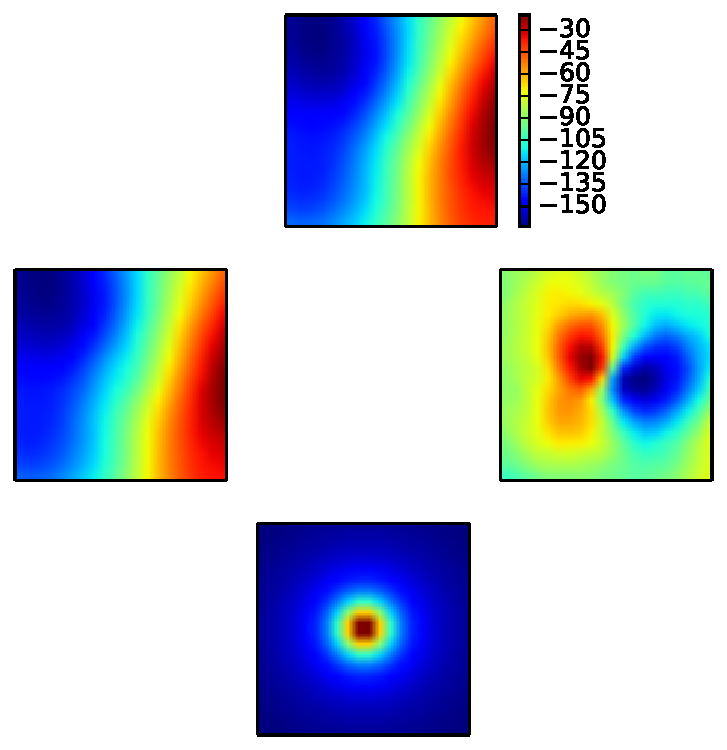
\includegraphics[width=\linewidth]{figs/schematic_rep.pdf}
\caption{Schematic representation of the QE. The top panel shows the observed CMB temperature map, which is then passed through the filters to obtain the large scale gradient map (left middle panel) and the small scale lensing map (right middle panel). The QE extracts the correlation between the gradient map and the lensing map to obtain the reconstructed lensing convergence profile shown in the bottom panel.}
\label{fig:QE_schem}
\end{figure}
The schematic representation of quadratic estimator is shown in Fig. ~\ref{fig:QE_schem}. 
The top panel is the \smallboxsize \; cutout of the observed temperature map. 
%\footnote{note that it is an ideal case, we haven't used either experimental noise level or foregrounds which are present in the real data}.
The observed temperature maps is then filtered in the fourier space (using Eqs. ~\ref{eqn_filters} and ~\ref{eqn_filter1}) to obtain the filtered gradient and lensed maps, shown in middle right and left panels respectively.
The lensing convergence map is reconstructed by extracting the correlations between the lensing and the gradient map, which is shown in the bottom panel.
 Note that Fig. ~\ref{fig:QE_schem} is for only idealised simulations and we have neither included experimental noise nor foregrounds.

  \subsection*{mitigating the magnification bias:}
\begin{figure}[ht]
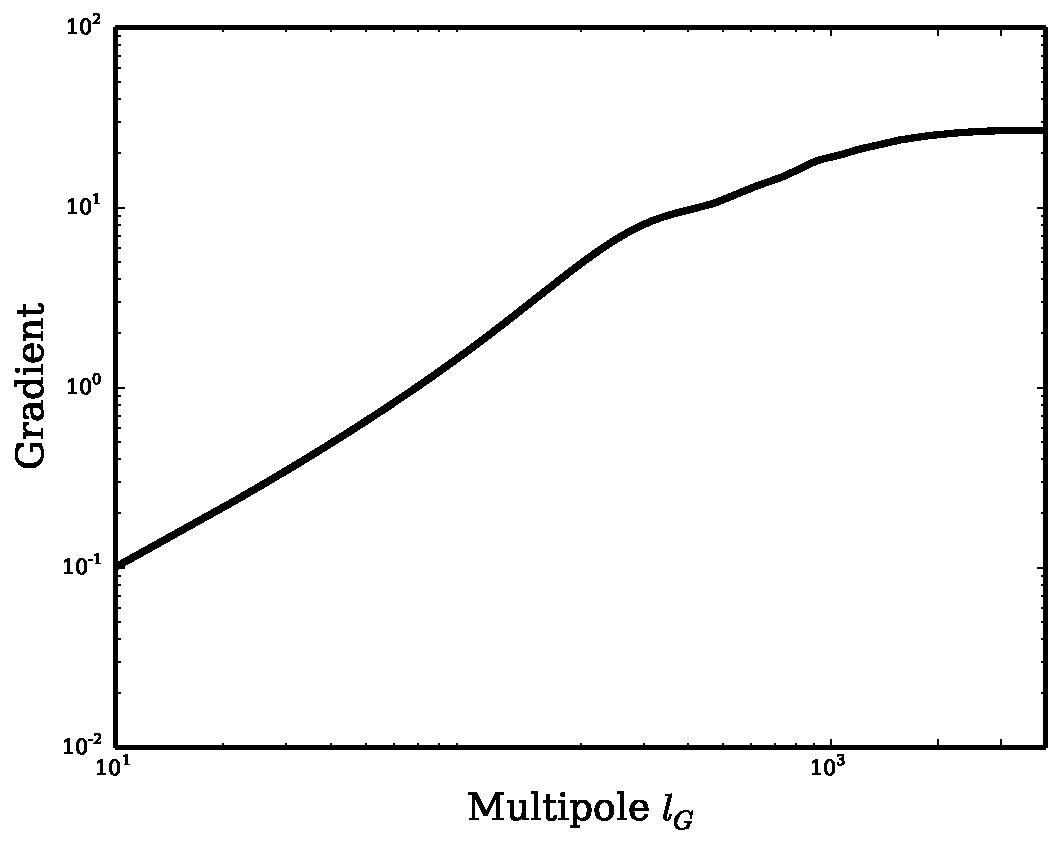
\includegraphics[width=\columnwidth]{figs/gradient_cut.pdf}
\caption{Gradient of temperature field as a function of the maximum of a top hat low pass filter (LPF), $l = l_{G}$. The curve has plateau above $l_{G} > 2000$. Low pass filtering the gradient map with $l_{G}<2000$ mitigates the magnification bias without affecting the SNR.}
\label{fig:gradient_cut}
\end{figure}
Galaxy cluster magnifies the background image and decreases the observed temperature gradient behind it, which leads to a low bias in the lensing reconstruction.
The bias is due to the overlap in scales between the unlensed gradient field and lensed temperature field. 
Though wiener filter reduces the bias, the filter cannot remove the bias.
We can reduce the bias further by exploiting the prior knowledge on unlensed CMB power spectrum.
 From Fig.~\ref{fig:gradient_cut}, which shows the unlensed rms gradient as a function of a top hat low pass filter, it is evident that most of the power for the gradient map comes from scales below $l \le 2000$.
 By low pass filtering the gradient map $l \le 2000$ the SNR of the gradient map is negligibly affected.
 On these scales, the lensing correction is only tiny for a typical cluster. 
 We get a clean separation between the unlensed gradient and the lensed temperature field by modifying the filter in Eq.~\ref{eqn_filters}  to % with almost no loss in SNR (signal to noise ratio) which is equivalent of modifying the gradient filter (Eqn. ~\ref{eqs_filters})to 
 \begin{equation}
 W^{TT}_{l} =  
    \begin{cases}
        \widetilde{C}^{TT}_{l}(C^{TT}_{l} + N^{TT}_{l})^{-1} \quad l \le l_{G}\\
        0, \quad otherwise
    \end{cases}
\end{equation}
where $l_{G}$ = 2000. 

It is worth here to note that the magnification bias depends on the mass of a galaxy cluster - higher the mass higher the bias. While $l_{G} = 2000$ should be sufficient to low mass clusters, for rare massive clusters (few times $10^{14} M_{\odot}$) even the large scale modes are significantly affected by the magnification bias and more aggressive $l_{G}  = 1000$ yields a bias free reconstruction \citep{hu07}. 
  
 
\subsection{SZ induced bias}
\label{sec_sz_induced_bias}
Though SZ is a small spectral effect, it is still much higher than the lensing signal. 
 It is an order of magnitude larger than the lensing signal inducing a significant systematic and statistical uncertainty if not taken into account. 
Fig ~\ref{fig:SZ_effect} shows the effect of SZ on the lensing convergence profile. 
 %In the left panel of figure 
% We show the stacked lensing convergence profile of 1000 clusters each with a mass of $2 \times 10^{14}$ $M_{\odot}$ and at a redshfit of $z= 0.7$.
 We simulate 1000 clusters each with a mass of $2 \times 10^{14}$ $M_{\odot}$ and at a redshfit of $z= 0.7$.
 To these simulated clusters we add experimental white noise noise level of 3\ukam\ 
. On the top panels we show the stacked lensing convergence profile of these 1000 clusters - the left panel is without adding SZ and the right panel is after adding \citet{arnaud10} SZ profile. % to these 1000 clusters. %and on the right panel is with the SZ.  
 As can be inferred from the plot, the presence of SZ induces a semi-resolved negative signal decrement (blue blob) in the center resulting in a negative bias.
 In the bottom panel we have the radial profiles of the two-dimensional kappa profiles.
 The blue (green) solid curve represents the radial lensing convergence profile with (without) SZ; the solid black curve represents the theoretical model.
 % without SZ in solid green and with SZ in solid blue curves.
 %As can be inferred from the plot the green curve matches with model within statistical uncertainty, however, the solid black is biased low.
%The major foreground in CMB cluster lensing analysis is SZ effect.
%SZ effect is an order of magnitude greater than lensing signal; if not taken into consideration it induces systematic bias and variance in the final convergence maps.
%In the next section we describe the modifications of QE in order to eliminate the SZ induced bias and in the next chapter we discuss the method to reduce SZ induced variance.

 \begin{figure}[ht]
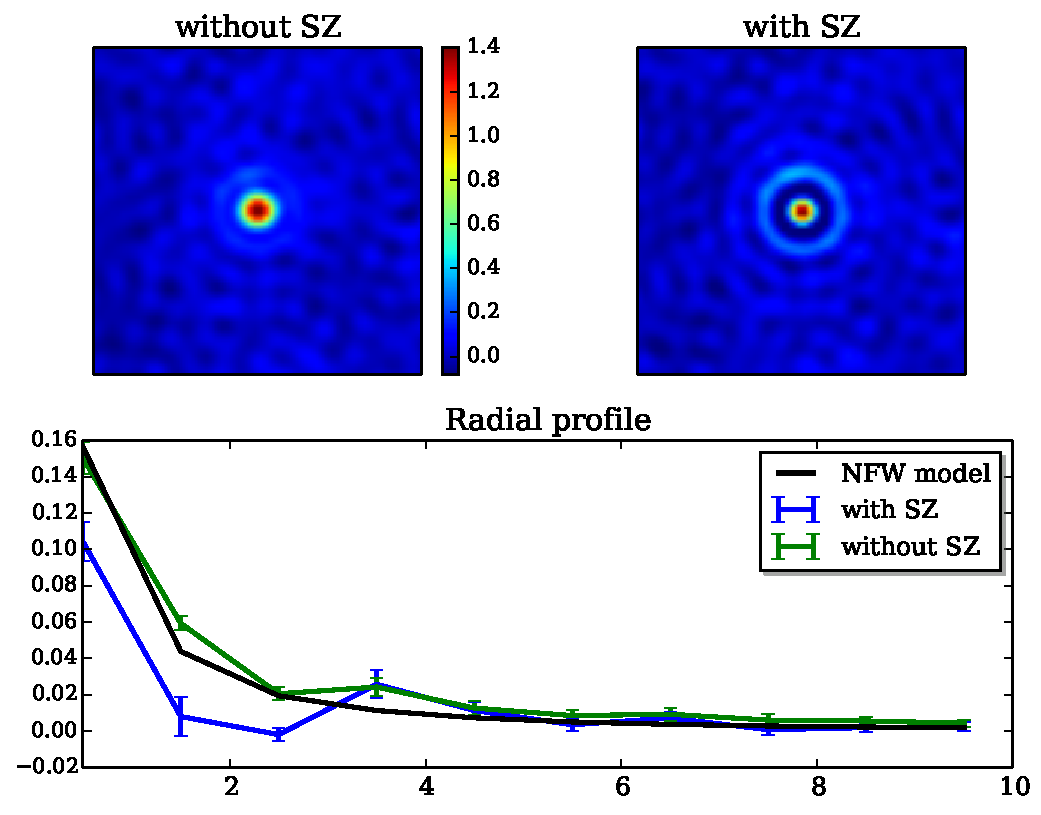
\includegraphics[width=\linewidth]{figs/tSZ_effect_on_lensing.pdf}
\caption{Effect of SZ on lensing convergence profile. On the top panel we show the lensing convergence profile for a stack of 1000 cluster each at a mass of $M_{200m}= 2*10^{14}  M_{\odot}$ and a redshift of $z = 0.7$ with experimental white noise level of $3\ukarcmin$; left panel is without SZ and right panel is with SZ. On the bottom panel we have radial profile of the same in solid blue (without SZ) and green (with SZ) curves; black curve is the radial profile of the input NFW profile. }
\label{fig:SZ_effect}
\end{figure}
%\subsection{modified quadratic estimator}
\subsection{Modified quadratic estimator}
While designed to pull out the lensing induced correlations, QE is equally sensitive to any other signal present in both G and L maps.
%The major systematic for lensing analysis is thermal Sunyaey -Zel'dovich (SZ) effect, which is an order of magnitude greater than lensing signal biases the analysis if not taken into account. 
 SZ present in both the maps results in a low bias if not taken into account as shown in Fig. \ref{fig:SZ_effect}.
 Two methods have been discussed in literature to eliminate/mitigate the SZ bias:
 one of the ways to eliminate the SZ bias is by using SZ free maps, which are constructed by exploiting the spectral dependance of the SZ signal.
 %Previous studies either used a SZ free map or a more stringent low pass filtering of the gradient map.
 %SZ is frequency dependent signal and hence we can use multiple frequency channels to eliminate SZ. 
 However, this results in an increased statistical uncertainty in the reconstructed convergence profile.
 Another way to mitigate the bias is by using a more stringent low pass filter on the gradient map, wherein a robust separation of scales between gradient map and small scale map reduces SZ correlation.
 While this can reduce the bias significantly,  poor gradient estimation results in an increased statistical uncertainty.

 
 During this thesis, we came up with a novel approach to completely remove the SZ bias. 
 Any foreground signal which is present in both the maps (gradient and lensing) will lead to a systematic bias; therefore, removal of the foreground signal in one of the maps (either gradient or lensing map) should eliminate the bias completely.
  As shown in Fig.~\ref{fig:gradient_cut}, most of the gradient estimation comes from multipoles $l \le 2000$ where CMB is not limited by experimental noise.
  The natural choice would be to eliminate SZ in the gradient map by using linear combination of different frequencies. 
  In the mQE, Eqn. ~\ref{grad_map} becomes,
  \begin{equation}
   G(\hat{n}) = \nabla (\int\frac{d^{2}l}{(2\pi)^{2}} e^{il .\hat{n}} W^{TT}_{l} T^{SZ -free}_{l}   )
  \end{equation}
  where $T^{SZ-free}_{l} $ is an SZ-free map obtained by linear combination of different frequency channels. Also the Eqns. ~\ref{eqn_filter1} and ~\ref{eqn_filters} are modified to 
  \begin{eqnarray}
    \begin{aligned}
   W^{TT}_{l} =  
    \begin{cases}
        \widetilde{C}^{TT}_{l}(C^{TT}_{l} + N^{TT-SZ-free}_{l})^{-1} \quad l \le l_{G}\\
        0, \quad otherwise
    \label{mdf_eqns}
    \end{cases}\\
 W^{T}_{l} = (C^{TT}_{l} + N^{TT}_{l})^{-1}.
 %\label{grad_filter}
 \label{eqs_filters}
 \end{aligned}
  \end{eqnarray} 
  where $N^{TT-SZ-free}_{l}$ is noise power spectrum of the SZ-free map obtained after deconvolving the experimental beam and transfer function. 
  
  \section{Cluster cutouts} %and model fitting}
 
% In this section first we describe the extraction of cluster cutouts from SPTpol maps in \ref{sec:cluster_cutouts}, followed by model fitting in \ref{sec:model_fitting}. 

 
\label{sec:cluster_cutouts}
 We extract 300\arcmin\ square box from the data temperature maps at the cluster locations. 
The boxsize is much larger than the virial radius of the cluster; however, it is necessary to robustly approximate the background gradient. 
This is because much of the gradient power comes from large scale modes, reducing the analysis to a smaller box will reduce the SNR of the mass estimation. 
These cutouts are then passed through the pipeline to extract lensing convergence profile, after which we limit the modelling and likelihood calculations to 10\arcmin\ box around a cluster to reduce the computational complexity.

As mentioned before, the lensing signal is weak for individual cluster and we need to stack lensing convergence profiles to increase the SNR of detection.
 Thus the stacked convergence map is simply: 
 \begin{equation}
 \hat{\kappa} = \frac{\sum_j  w_j \left[ \hat{\kappa}_{j} - \left< \hat{\kappa}_{j} \right> \right]}{\sum_j w_j} - \hat{\kappa}_{\rm MF},
 \end{equation}
% where the subscript $j$ refers to an individual cluster and the weighting scheme $w$ is described below.
 where $\hat{\kappa}_{j}$ refers to the reconstructed convergence map of $j^{th}$ cluster %satisfying $\left< \hat{\kappa}{\rm C}_{j} \right> = 0$ 
 and  $w_{j}$ is weight assigned to the $j^{th}$ cluster.
%From the stacked map, we remove all modes above the experimental beam scale and the modes corresponding the data filter function. %of $\theta_{\rm FWHM}\sim 1.^{\prime}2$. 
%Relaxing this filter does not contribute much to the \snr{} as those modes are either dominated by foregrounds or noise. 
We remove an estimate of the mean-field $\hat{\kappa}_{\rm MF}$ from this stacked convergence map.
The mean-field arises because of two following reasons:
\begin{itemize}
\item  the temperature maps are apodized using a Hanning window with a $10^{\prime}$ edge taper to reduce edge effects which induces undesired mode correlation.
\item the presence of inhomogeneous noise in the survey region.
\end{itemize}
We obtain the mean field bias by stacking the convergence maps reconstructed at \howmanyrandomsforMF{} random locations in the maps. 


{\it Weighing scheme:}  We completely eliminated the SZ-induced bias by using SZ-free maps. However, the SZ present in the lensing map induces extra variance.
The SZ variance is proportional to the SZ brightness and scales roughly as $M^{5/3}$.
%For example, the lensing signal of a cluster is proportional to its mass $M$ while the SZ signal scales roughly as $M^{5/3}$.
We will discuss in detail a refined mQE to suppress the SZ induced variance in the next chapter ~\ref{ch:template}.
 Here we just down weigh the clusters based on their SZ variance.
We decompose the weights assigned for each cluster into two components: inverse noise variance weight and SZ variance weight. 
 
 
 The inverse-noise-variance weight, $w_{k}$, is obtained from the data.
  We pass data cutouts through pipeline to get the lensing convergence profile.
 As most of the lensing signal is within 10\am\ of the cluster center, the variance outside 10\am\ should be identical to the inverse-noise-variance.  
 We take the standard deviation in the reconstructed convergence maps in a ring between $10^{\prime}$ and $30^{\prime}$ around the cluster center and define it as $\sigma_{\kappa}$ . 
%The noise in convergence is proportional to the noise in the associated gradient map and increases, as expected, when $\ell_{\rm G}$ is reduced.
%While our method completely eliminates the SZ-induced lensing bias, the presence of SZ signal in the second map tends to increase the variance in the final convergence maps. 
%The noise is proportional to the SZ brightness and, as expected, is higher for massive clusters.
%For example, the lensing signal of a cluster is proportional to its mass $M$ while the SZ signal scales roughly as $M^{5/3}$.
%Given that our cluster sample contains $\le 4\%$ clusters with richness $\lambda \ge 60$ (\mbox{\mvir\ $\sim 5.2\ \times$ \munits} at $z=0.5$), this extra noise does not completely average out and our results are sample variance limited.

The second %\footnote{We note that for the mean-field reconstructed from random locations, we only apply the weight $w = 1/\sigma_{\kappa}^2$ for stacking.} 
 weight comes from the noise in the convergence maps due to the presence of SZ signal in the lensing map.%, the \sptpol{} 150 GHz map.
We obtain this second set of weights, $w_{\rm SZ}$, using simulations. 
For every cluster in the sample, we reconstruct the convergence profile using a simulated SZ-free gradient map and the lensing map with SZ signal assuming an Arnaud profile \citep{arnaud10} with a log-normal scatter of 20\% in the $Y_{SZ}-M$ relation. 
We pass these simulated cutouts through our pipeline and turn off cluster lensing as the objective here is to only get an estimate of the SZ-induced noise in the convergence maps.
%A total of 25 simulations were used to get the noise estimate for each DES cluster and we perform two sets of simulations: one with \sptpol{} SZ-free gradient map and the other with \lgmca{}.
A total of 25 simulations are used to get the noise estimate for each cluster.
The weights are estimated as
%using the inverse noise variance 
$w_{\rm SZ} = 1/\sigma_{\rm SZ}^{2}$, where $\sigma_{\rm SZ}$ is the standard deviation of the `null' convergence map within an angular distance of $10^{\prime}$ from the cluster centre.
%The errors increase with richness and take a power law form parameterized as $\sigma_{\rm SZ}(\lambda) =  \sigma_{0}\lambda^{\alpha}$ with values $(\sigma_{0}, \alpha) = (0.0045, 1.55)$ for the \sptpol{} $\times$ 150 GHz and $(\sigma_{0}, \alpha) = (0.0066, 1.39)$ for the \lgmca{} $\times$ 150 GHz cases. \pending{(Pending SR: I must think a bit more if it makes sense that the weights change when the gradient map (/noise) changes.)}
%The errors increase with richness and take a power law form parameterized as $\sigma_{\rm SZ}(\lambda) =  \sigma_{0}\lambda^{\alpha}$ with values $%%%commentingthisoutfornow(\sigma_{0}, \alpha) = \pending{(0.0045, 1.55)}$.
%(\sigma_{0}, \alpha) = (0.0045, 1.55)$.
%The results are unchanged if we derive the weights using the SZ signal from \cite{sehgal10}.
%The standard deviations vary by up to a factor of \pending{six}, based on the local survey noise and point source mask, although 90\% of the standard deviations are within a factor of \pending{two} of each other. 
 % We choose to use uniform weights across the N-cluster sample, $w_j = 1/N$. 

The total weight is now:
 \begin{equation}
 w = \frac{1}{\sigma_{\kappa}^{2} + \sigma_{\rm SZ}^{2}}.
\label{eq_cluster_weight}
 \end{equation}
 As expected, introducing $w_{\rm SZ}$ down weighs the massive clusters as the SZ variance is $\sim$ $M^{5/3}$.
 This reduces the contribution of clusters with $\sigma_{\rm SZ} > \sigma_{\kappa}$ resulting in a decrease of SNR. 
 The number of clusters with dominate SZ variance depend on the mass distribution of cluster catalog and the experimental noise level (which will be discussed in detail in next chapter \ref{ch:template}).
 One of the alternative ways to tackle this problem would be to swap the maps, by using SZ-free lensing map and single frequency channel for gradient map.
However, this still won't help us in gaining SNR as the SZ-free maps have higher noise level than a single frequency map. 
%The increase in the noise level of SZ-free channel depends on the noise level and beam size of different frequency channels used. 
For SPTpol like experiment which observes sky in 90 and 150 GHz the SZ-free noise level is 3 $\times$ larger than 150 GHz noise level. %noise level of SZ-free maps is 3 $\times$ the noise level of 150GHz maps.  
% in a minimal gain as the
  % in the two legs of the QE (i.e gradient and lensing map) for massive clusters. 
%As expected introducing $w_{\rm SZ}$ down weighs the massive clusters as the SZ variance is $\sim$ $M^{5/3}$.
%This reduces the contribution of clusters with $\lambda \ge 60$ to less than 1\% in the final stacked sample. 
%This is why the change in gradient-map LPF scale to \mbox{$\ell_{\rm G} = 1000$} from the fiducial \mbox{$\ell_{\rm G} = 2000$}
%for these clusters (see \S\ref{subsec_QE_modificaltion}) has negligible effects in our final results. 
%Note that we have only 40 clusters above $\lambda > 40$ and down weighing doesn't significantly reduce the SNR. 
%However, for future low noise surveys down weighing will suppress the contribution of large number of clusters.
%An alternative would be to swap the maps in the two legs of the QE (i.e. the 150 GHz map for the gradient estimation and the SZ-free map to reconstruct lensing map) for clusters with \mbox{$\sigma_{\rm SZ} > \sigma_{\kappa}$}, which is approximately true for clusters with $\lambda > 40$. But this results in a minimal gain as the \sptpol{} SZ-free map has a higher noise ($\times3$) compared to the \sptpol{} 150 GHz maps. 
%In the next chapter, we discuss the template fitting approach used to reduce the SZ variance significantly.
%Some other approaches to handle the additional noise from the SZ signal include (a) rotating the reconstructed lensing map based on the direction of the background CMB gradient and fitting for the SZ-noise, (b) removing a matched-filter estimate of the SZ-signal from the 150 GHz map before passing the map into the QE. We will explore such possibilities in detail in a future work (Patil S. et al. 2019, in preparation).
 \section{Model Fitting}
 \label{sec_model_fitting}
 With cluster cutouts obtained from \S\ref{sec:cluster_cutouts} and the method to extract convergence profile (\S\ref{sec_method}) in hand, we can fit the model to the observed convergence.
To obtain the mass of the cluster, we need to compare the observed lensing profile to the convergence model generated using an assumed halo mass profile.
 The observed lensing convergence profile of cluster has contributions from its own halo density ($\kappa_{1h}$) as well as from the correlated structures along the line of sight known as two halo term ($\kappa_{2h}$) \citep{oguri11}.
 For $\kappa_{1h}$, we assume the galaxy cluster density to follow Navarro Frenk White (NFW,\citep{navarro96}) profile and in \ref{mqe_sec_systematics} we quantify the robustness of this assumption by using Einasto profile \citep{einasto89}.
 A NFW halo profile is characterized by its scale radius $R_{s}$, the dimensionless concentration parameter c, and the dimensionless characteristic over-density $\delta_{c}$.
 The lensing convergence profile for NFW is obtained as discussed in the previous chapter \S\ref{sec_def_field} which we represent as $\kappa_{1h}(\theta)$. We also add two halo term ($\kappa_{2h}$) \citep{oguri11} to the  $\kappa_{1h}(\theta)$ to get $\kappa(\theta)$.
%\iffalse{
 %The characteristic over density is defined as the ratio of central cluster density to the critical density of the Universe at the cluster redshift.
 %In terms of these quantities the NFW halo density profile is written as 
 %\begin{equation}
 %\rho(r) = \frac{\delta_{c}\rho_{crit,z}}{(\frac{r}{R_{s}})(1 + \frac{r}{R_{s}})^{2}}
 %\end{equation} 
 %where $\rho_{crit,z}$ is the critical density of the Universe at cluster redshift.
%
 %The lensing convergence profile is the ratio of surface mass density to the critical surface density of the Universe at cluster redshift, $\kappa(x) = \frac{\Sigma(x)}{\Sigma_{crit}}$, where
% \begin{eqnarray}
 %\Sigma(x) = 2 \int^{\inf}_{0} \rho(r) ds\\
 %\Sigma(crit) = \frac{c^{2}}{4\pi G} \frac{D_{CMB}}{D_{clus} D_{CMB,clus}} 
 %\end{eqnarray} 
%Here r is the distance from the center, x is the corresponding projection on the plane,$D_{CMB}$ and $D_{clus}$ are the comoving distances to the CMB and galaxy cluster respectively; $D_{CMB,clus}$ is the distance between the CMB and the cluster.
%}fi
With the model prediction in hand, we can then write down the likelihood of observing the data convergence profile as: 
\begin{equation}
-2\ln\mathcal{L (\hat{\kappa}(\theta)| \rm{M}}) = 
\sum_{\theta, \theta^{\prime} = 0}^{10^{\prime}}\left[\hat{\kappa}(\theta) - \kappa(\theta)\right] \hat{{\rm C}}_{\theta, \theta^{\prime}}^{-1} \left[\hat{\kappa}(\theta^{\prime}) - \kappa(\theta^{\prime})\right]
%\sum_{\theta = 0}^{10^{\prime}}\left[\hat{\kappa}(\theta) - \kappa(\theta)\right] \hat{{\rm C}}^{-1} \left[\hat{\kappa}(\theta) - \kappa(\theta)\right]^{T},
\label{eq_QE_likelihood}
\end{equation}
where $\hat{\kappa}(\theta),\ \kappa(\theta)$ are the azimuthally averaged radial profiles of the stacked data and model convergences respectively, binned in 10 linearly spaced intervals with $\Delta\theta = 1^{\prime}$. % up to $10^{\prime}$.


We use the jackknife re-sampling technique to obtain the covariance matrix. We divide the \sptpol{} 500 \sqdeg\ region into $N=500$ sub-fields and estimate the covariance matrix for the radially binned convergence profile as 
\begin{equation}
%\hat{{\rm C}}_{\theta, \theta^{\prime}} = \frac{N-1}{N} \sum\limits_{j=1}^{N = 500} \left[\hat{\kappa}_{j}(\theta) - \left<\hat{\kappa}(\theta)\right>\right] \left[\hat{\kappa}_{j}(\theta^{\prime}) - \left<\hat{\kappa}(\theta^{\prime})\right>\right]^{T}.
\hat{{\rm C}} = \frac{N-1}{N} \sum\limits_{j=1}^{N = 500} \left[\hat{\kappa}_{j}(\theta) - \left<\hat{\kappa}(\theta)\right>\right] \left[\hat{\kappa}_{j}(\theta) - \left<\hat{\kappa}(\theta)\right>\right]^{T},
\label{eq_JK_cov}
\end{equation}
where $\hat{\kappa}_{j}(\theta)$ is the azimuthally binned stacked convergence of all the clusters in the $j^{th}$ sub-field and  $\left<\hat{\kappa}(\theta)\right>$ is the ensemble average of all the 500 sub-fields.
 %as in Eq. (\ref{eq_JK_cov}). 
We test this approach by alternatively estimating the covariance matrix using 500 realizations of the random convergence stacks. 
We do not note any significant differences between the uncertainties estimated using the two approaches. 
We apply the \citet{hartlap06} correction to $\hat{{\rm C}}^{-1}$ to account for the noise in covariance estimation due to the finite number of jackknife re-sampling.
%We take the parameter uncertainties to be the standard $1\sigma$ errors estimated using the statistic \mbox{$\Delta \chi^2 = 2\ln \mathcal{L}(\Theta) - 2\ln \mathcal{L}(\Theta_{\rm fit})$} where $\Theta \in [A, \alpha]$.
%We take the parameter uncertainties to be the standard $1\sigma$ errors estimated using the statistic \mbox{$\Delta \chi^2 = 2\ln \mathcal{L}(M) - 2\ln \mathcal{L}(M_{200m})$}.
%%Throughout this work, we sample the likelihood space and compute the parameter uncertainties $1\sigma$ from the 16$^{th}$ and 84$^{th}$ percentiles of the resultant samples.
%to be the standard $1\sigma$ errors estimated using the statistic \mbox{$\Delta \chi^2 = 2\ln \mathcal{L}(M) - 2\ln \mathcal{L}(M_{200m})$}.


% can enhance other frequency dependent foregrounds. This  can lead to: (a) an increased variance in the final lensing signal; and more importantly (b) enhance the emission due to radio/dusty galaxies that live in the cluster. The latter effect can lead to a biased lensing signal as it is correlated to the galaxy cluster of interest. This is expected to be particularly large for massive clusters. We use the \cite{sehgal10} simulations to estimate this bias (see Fig. \ref{fig_QE_sehgal_sims}) and impose a conservative cut of $\lambda \ge 60$ to remove 125 (88) massive clusters in our analysis from the full (cosmology) sample of the DES RM catalog.

While fitting model to the real data we need to account for mis-centering of cluster, otherwise the results are biased low. 
For instance \citet{rykoff16} compared the centroids DES RM clusters with SZ \citep{bleem15} and X-ray observations and found a fraction, $f_{mis} = 0.22 \pm 0.11$, of the DES clusters to be mis-centered by $\sigma_{R}$, which is a fraction of the cluster radius $R_{\lambda} = (\lambda/100)^{0.2} \: h^{-1}$.
They further modelled the mis-centering as a Rayleigh distribution with $\sigma_{R} = c_{mis} R_{\lambda}$ where $\ln c_{mis} = -1.13 \pm 0.22$.
 Mis-centering smears the convergence profiles and we use the prescription provided in Eq. (34) of \citet{oguri11} to account for cluster mis-centering in the real data. %In addition to the cluster mis-centering, for real data we also need to account for the experimental filter and beam transfer functions. 
As we will see in \S\ref{sec_data}, we lose some modes due to data filtering and the experimental beam size. The modes corresponding to the filtering and beam scale are removed from the model before fitting to the real data.
 
  
\section{Data}
\label{sec_data}
In order to estimate the mass of a cluster catalog, we need the cluster location and the CMB map corresponding to the cluster location.
 Both catalog and CMB map can come from the same experiment (for example SZ surveys) or from different experiments whose survey areas overlap.
In our case we used data sets from two different experiments: CMB maps from South Pole Telescope explained in \S\ref{sec_SPT} and 
optical cluster catalog from Dark Energy Survey explained in \S\ref{sec_DES}

\subsection{South Pole Telescope}
\label{sec_SPT}
South Pole Telescope (SPT) is a 10 meter diameter, wide field, offset Gregorian telescope \citep[SPT,][]{ carlstrom11,padin08} located at the Amundsen-Scott South Pole station.
The SPT has been operating since early 2007 and has completed two surveys so far: SPT-SZ (2007 -2011) and SPTpol (2012-2016).  
Extremely dry and stable atmosphere of the South Pole makes it one of the best available sites on Earth for observing at millimeter and sub-millimeter wavelengths. 

\subsubsection*{\sptpol{} {\rm 500} deg$^{2}$ survey}\label{sec_sptpol}
SPT installed a polarisation sensitive camera, \sptpol{}, during the austral summer of 2011-2012. 
The \sptpol{} focal plane consists of 1536 polarization-sensitive transition edge sensor bolometers (360 at 95 GHz and 1176 at 150 GHz)\citep{austermann12}.%is the second polarisation sensitive camera installed on the \mbox{10-meter} South Pole Telescope.
%The \sptpol{} focal plane consists of 1536 polarization-sensitive transition edge sensor bolometers (360 at 95 GHz and 1176 at 150 GHz) \citep{austermann12}.
%enabling polarization observations \citep{austermann12}.
The \sptpol{}  surveyed 500~deg$^{2}$ of southern sky spanning fifteen degrees of declination, from -65 to -50 degrees, and four hours of right ascension, from 22h to 2h. 
In this section we briefly summarize the \sptpol{} observation strategy, map making, and beam characterization; we suggest interested reader to refer \cite{henning18} for further details. 
%In this work we use the temperature (T) and polarization (Stokes Q and U) maps of the CMB from observations between April 2013 to September 2016 in the frequency bands 95 GHz and 150 GHz. 

In this work, we use CMB temperature maps from observations between April 2013 and September 2016 in the frequency bands centered at approximately 95 GHz and 150 GHz.  Over this period, SPT used two different scanning strategies to observe the field. From April 2013 upto May 2014 SPT observed the field in lead-trail strategy and for the rest of the observation period SPT adopted full-field strategy. In lead trail strategy the field is split into two halves in right ascension - lead-field and trial-field. The lead-field is scanned first for a period of 2 hours, immediately followed by a 2 hour trail-field scan.  During lead-trail strategy the scan speed and elevation steps are set such that the entire observation occurs over the same azimuth range. In order to increase sensitivity at large angular scales, SPT adopted full-field strategy for the rest of its observation period, where constant-elevation scans were made across the entire range of right ascension over 2 hour period.


%\pending{include scanning strategies}
The telescope beam and pointing solutions were characterized by observing Venus.
  SPTpol made seven observations of Venus. From these seven observations we calculate the 21 independent cross power spectra and take the average to  characterize beam, $B_{l}$.
 The beam covariance is estimated as the noise variance of these 21 independent cross-spectra. 
 Broadening of the beam is caused by two sources: rms pointing error and finite size of Venus.
 During the analysis it was found that broadening due to the finite size of Venus (which was $\sim$ 11 arc seconds) is negligible.
The final telescope beam along with the pointing jitter roughly corresponds to a $\theta_{\rm FWHM} = 1.^{\prime}22\ (1.^{\prime}7)$ Gaussian for the 150 (95) GHz dataset.

\begin{figure}[!ht]
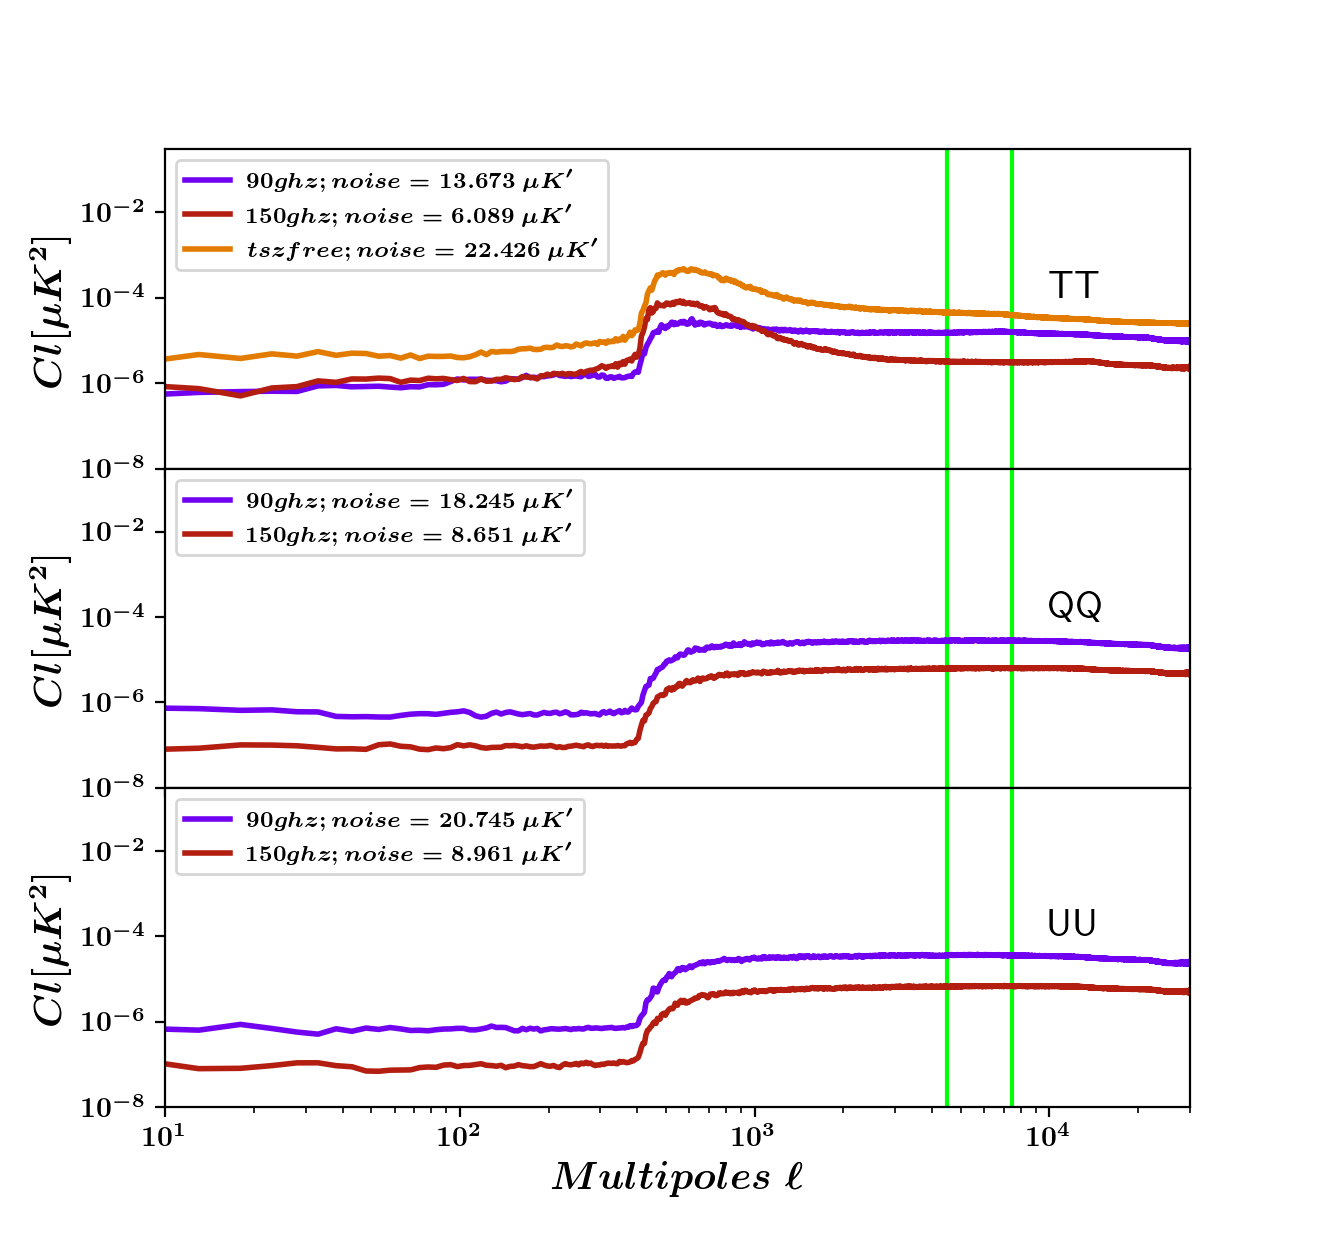
\includegraphics[width= \columnwidth]{figs/noise_Cls_sanjay_maps_20170603.png}
\caption{SPTpol noise power spectrum of temperature and polarisation maps. The vertical green solid lines are the multipole range across which the corresponding white noise level is calculated.}
\label{noise_ps}
\end{figure}

The raw data is composed of digitised time-ordered data (TOD) for each detector that are converted into CMB temperature units. %% using a Planck-based calibration factor. 
We bin the TOD into two different maps using a flat-sky approximation in the Sanson-Flamsteed projection \citep{calabretta02, schaffer11}. 
To construct the first map (lensing map), in which we aim to reconstruct the small-scale lensing signal ($L(\hat{n})$), we remove large-scale modes $\ell \le 300$, bandpass filter the TOD in the range of approximately $300 \le \ell_{x} \le 20,000$, and bin them into 0.\am5\ square pixels.
For the second map (SPTPol SZ-free gradient map), intended for estimation of the large-scale CMB gradient ($G(\hat{n})$), we apply minimal TOD filtering by only removing modes below $\ell_{x} \le 30$, and bin them into 3\am\ square pixels.
While we only use the data from the 150 GHz channel for the first map, the latter is a SZ signal cleaned map produced by linearly combining the 95 and 150 GHz channels. 
We use this SZ-free map to reconstruct the background gradient of the CMB at the cluster locations.
%As we will see later in \S\ref{sec_method_QE}, the gradient estimation using the SZ-free map helps in removing the SZ-induced lensing bias.
The minimal filtering on this map allows us to recover large-scale modes which indeed helps in a better estimation of the background gradient.
The 0.\am5{} resolution of 150 GHz temperature map has a white noise level of \mbox{$\Delta_{\rm T} = $ 6 \ukam} estimated using a jackknife approach. %estimated within the multipole band $4500 \le \ell \le 7500$.
The low-resolution SZ-free combination is noisier with \mbox{$\Delta_{\rm T} \sim $ 22 \ukam}.

Fig. ~\ref{noise_ps} shows the noise power spectrum of temperature and polarisation maps. 
Top panel in the figure represents the temperature noise power spectrum and the bottom two panels correspond to polarisation stokes Q and U maps. 
The purple and maroon curve in all the panels correspond to noise spectrum of 90 and 150 GHz channels respectively.
The orange curve in the top panel represents the noise power spectrum of the tSZ-free maps obtained by using linear combination 90 and 150 GHz channels. 
In all the three panels the vertical green curves represent the multipole range across which the white noise level is calculated.


%%%\pending{Pending: SR: Should we quote this? Can we trust this number?}
%\section*{Cosmic Microwave Background cluster lensing}
\subsection{DES and the {\rm \RM} catalog}\label{sec_DES}
The Dark Energy Survey (DES) was a $\sim$5000 \sqdeg, optical to near-infrared survey conducted using the Dark Energy Camera \citep{flaugher15} mounted on the 4-meter Victor Blanco telescope at Cerro Tololo Observatory in Chile and has recently finished its survey. 
For this analysis, we use the cluster catalog obtained from the first three years of DES observations, which completely overlaps the \sptpol{} 500\,deg$^{2}$ survey. 

%The cluster catalog was derived using the RM algorithm \citep{rykoff14}  from the DES photometric datasets. 
The cluster catalog was derived using the redMaPPer (RM) algorithm \citep{rykoff14}.
RM is an optical cluster-finding algorithm which detects candidates by identifying over-densities of luminous red galaxies with luminosity greater than 20\% of $L_{*}.$
%Milky Way ($0.2L_{*}$). [I DON'T THINK THIS IS ACTUALLY THE DEFINITION OF L* (TC\cite{mcclintock18})]
It is based on our understanding that galaxy clusters are agglomerations of galaxies containing old and subsequently red stars. 
The algorithm iteratively assigns membership and centering probabilities for each red galaxy identified as belonging to a cluster candidate. 
A weighted sum of the membership probabilities, richness $\lambda$, is assigned to each candidate.
The centre comes from the galaxy with the highest centering probability.
The DES RM catalog contains two samples: a flux-limited sample and a volume-limited sample. 
The flux-limited sample has more high-redshift clusters detected from deep fields in the survey. 
On the other hand, the volume-limited sample is independent of survey depth, complete above a luminosity threshold \citep{mcclintock18}, and normally preferred for cosmological analysis.
% (hereafter referred to as the volume-limited sample).
See \citet{rykoff16} for more information on the application of RM to the DES survey data.

The RM cluster catalog version employed in this analysis is Y3-gold (\whichcatversion). 
The \whichyear{} gold catalogue is based on the previous catalog from the Year-1 data \citep{drlica-wagner17} with some updates as described in \citet{morganson18}.
The catalog contains 54,112 clusters above richness $\lambda \ge 20$ in the flux-limited sample and 21,094 clusters in the volume-limited sample. % \pending{(Pending: Cite DES Y3 cat. paper)}. 
Of these, 5,828 (2,428) clusters from the flux(volume)-limited sample lie within the \sptpol{} 500 \sqdeg{} survey  in the redshift range $0.1 \le z \le$ 0.95 (0.90). 
%We additionally remove clusters near the survey edges or within $10^{\prime}$ distance from a bright ($\ge 50$ mJy at 150\,GHz) point source.
We additionally remove clusters near the survey edges with more than 5\% masked pixels or within $10^{\prime}$ distance from any bright ($\ge 6$ mJy at 150\,GHz) point sources detected in the \sptpol{} temperature map.
%we use data/500sqdeg_bleem/quick_mm_point_source_file_150.0GHz_6.00000mJy.txt.
These cuts leave 4,003 (1,741) clusters with $\lambda \ge 20$ from the flux(volume)-limited sample with a median redshift of $\tilde{z}$ = 0.77 (0.48). 
The error in the cluster photo-$z$ estimates are small with $\hat{\sigma}_{z} = 0.01 (1+z)$ \citep{rozo15}.
%\pending{Finally, we impose a cut on the cluster richness and remove all clusters above $\lambda \ge 60$ that removes \pending{xx (xx)} from the full (cosmology) sample. This cut was motivated based on the results from Sehgal sims described in \S\ref{sec_xx_xx}}.
%Cosmic Microwave Background (CMB) photons while passiang through intervening galaxy cluster gets lensed and we call this phenomenon as CMB-cluster lensing.
% Lensing remaps the unlensed CMB field based on the angular deflection caused by cluster gravitational potential.
 %In mathematical form CMB cluster lensing can be written as the equation below
 %\begin{eqnarray}
%T(\hat{\textbf{n}})& = & \widetilde{T} (\hat{\textbf{n}} + \vec{\alpha}(\hat{\textbf{n}}))\\
%Q(\hat{\textbf{n}}) & = & \widetilde{Q} (\hat{\textbf{n}} + \vec{\alpha}(\hat{\textbf{n}}))\\
%U(\hat{\textbf{n}}) & = & \widetilde{U} (\hat{\textbf{n}} + \vec{\alpha}(\hat{\textbf{n}}))
%\end{eqnarray}
%where $ \widetilde{T}$ is unlensed temperature field, $\widetilde{U}$ and $\widetilde{Q}$ are the unlensed polarisation fields.
%$\vec{\alpha}(\hat{\textbf{n}})$ denotes the deflection angle and is directly proportional to the mass of the galaxy cluster.

%Lensing signal by an individual cluster is too weak to detect, so we need to stack many clusters to obtain a significant signal.
 %For example, the lensing induced distortion due to a $2 \times 10^{14} \ M_{\odot}$ mass galaxy cluster  is $\sim 5.0$ and $0.5 \ \mu K$ in temperature and polarization respectively.
%In this chapter, we will discuss various methods available in literature to extract CMB-cluster lensing signal. 
%The chapter is organized as follows 
 \iffalse{
Note that the convergence model must be slightly modified to account for the uncertainties in the RM cluster centroids.
\citet{rykoff16} compared the centroids of DES RM clusters with SZ \citep{bleem15} and X-ray observations and found a fraction, $f_{\rm mis} = 0.22 \pm 0.11$, of the DES clusters to be mis-centered by $\sigma_{R}$, which is a fraction of the cluster radius $R_{\lambda} = (\lambda/100)^{0.2} h^{-1}$ Mpc. They further modelled the mis-centering as a Rayleigh distribution with $\sigma_{\rm R}  = c_{\rm mis} R_{\lambda}$ where ln $c_{\rm mis} = -1.13 \pm 0.22$.
Mis-centering ought to smear the convergence profiles and we use the prescription provided in Eq. (34) of \citet{oguri10} to account for the cluster mis-centering. We set \mbox{$f_{\rm cen} = 1- f_{\rm mis} =  0.78$} and $\sigma_{\rm s} = \sigma_{\rm R}/D_{\rm A}(z)$, where $\sigma_{\rm R}$ is picked from the Rayleigh distribution \citep{rykoff16}, and $D_{\rm A}(z)$ is the angular diameter distance at the cluster redshift $z$.
%After the mis-centering correction, we filter the model using the similar filtering scheme as the data using Eq. (\ref{eq_filter_TF}) and remove all modes $\ell \ge 6746$ below the \sptpol{} 150 GHz beam scale of $\theta_{\rm FWHM}\sim 1.^{\prime}2$. 
After the mis-centering correction, we filter the model using the approximation to the data filtering in Eq. (\ref{eq_filter_TF}) and remove all modes above the \sptpol{} 150 GHz beam similar to the data. % scale of $\theta_{\rm FWHM}\sim 1.^{\prime}2$. 
%We also correct the model for the cluster mis-centering as described in \S\ref{sec_clus_profile}. 
The filtered model of all the individual clusters is weighted (\S\ref{subsec_weights}), stacked, and radially binned. 
}\fi

\section{Pipeline verification}
\label{sec:pipeline_verfication}
%Before applying our pipeline to the date, we validated our pipeline using simulations.
In this section, we describe tests used to investigate the known and unknown systematic effects in the data and to validate the pipeline.
We describe simulations used in ~\ref{sims_used} followed by the test for unknown systematics through the ``curl'' null test (\S\ref{sec_null_tests}).
We then calculate the expected systematic error budget from known sources of systematic uncertainty (\S\ref{mqe_sec_systematics}). 

\subsection{Simulations}
\label{sims_used}
%We create Gaussian realizations of the ``lensed'' CMB power spectra from \texttt{CAMB} \citep{lewis00} for the fiducial \planck\ 2015 cosmology \citep{planck15-something}.
In this section, we describe the simulations used for the pipeline validation. % presented in \S\ref{sec_pipeline_validation}.
We calculate the large-scale structure lensed CMB power spectra for the fiducial \citet{planck15-13} cosmology using \texttt{CAMB} \citep{lewis00} 
and create \boxsize\ Gaussian realizations of the CMB temperature map with $0.^{\prime}25$ pixel resolution.%s\footnote{We have confirmed that the results are unchanged when going to smaller initial pixels.}
%We create these simulated T/Q/U maps with $0.^{\prime}25$ pixels in \boxsize\ boxes.\footnote{We have confirmed that the results are unchanged when going to smaller initial pixels.} 
 Given the small angular extent, these simulations are done in the flat-sky approximation. 
%Thus we can employ 2D Fourier transforms instead of spherical harmonic transforms, with the angular wavenumber $\bar{k}$ related to multipole $\ell$ by $\ell = |\bar{k}|$. 
These simulations are then lensed using the simulated galaxy cluster convergence profiles from the next section. 
We next apply the frequency-dependent foreground 
%(not lensed by the cluster) 
realizations. %(see \S\ref{sec_validation}). 
The simulated maps are convolved by the beam functions, and are rebinned to $0.^{\prime}5$ pixels to reduce the computational requirements. 

For realistic simulations, we must also account for the noise and the filtering applied to the real data. 
We add instrumental noise realizations corresponding to \sptpol{} maps (see \S\ref{sec_sptpol}).
We follow \citet{baxter18} and other SPT works and approximate the map filtering using a function of the form:
\begin{equation}
F_{\bar{\ell}} = e^{-(\ell_{1}/|\bar{\ell}|)^{6}}  e^{-(\ell_{2}/\ell_{x})^{6}} e^{-(\ell_{x}/\ell_{3})^{6}}.
\label{eq_filter_TF}
\end{equation}
We validate the robustness of this approximation in \S\ref{subsec_TF}.
For the small-scale lensing map, we set: \mbox{$\ell_{1}$ = 300}, \mbox{$\ell_{2}$ = 300}, and \mbox{$\ell_{3}$ = 20,000}. 
For the gradient map, we set: \mbox{$\ell_{1}$ = 0} (as the gradient map does not have an isotropic filter), \mbox{$\ell_{2}$ = 30}, and \mbox{$\ell_{3}$ = 3000}.

\subsection{``Curl'' null test}\label{sec_null_tests}

We perform a ``curl'' null test \citep{hu07} at \howmanyclustersinfullsample{} cluster locations from the DES RM \whichyear{} flux-limited sample.
Specifically, we replace the divergence of the gradient field, $\nabla \cdot [G(\bnhat) L^{*}(\bnhat)]$, in Eq. (\ref{mqe_convergence_eqn}) with the curl operator. 
Since the curl of a gradient field is zero, the reconstructed field should be consistent with zero unless there is a systematic bias in the data. 
The result of the curl test is shown in Fig. \ref{curl_test}. 
We radially bin the test results similar to the cluster stack as described in \S\ref{sec_model_fitting} and compare it to a null signal.
The test returns a probability to exceed (PTE) value of 0.26 consistent with a null signal.

\begin{figure}[ht]
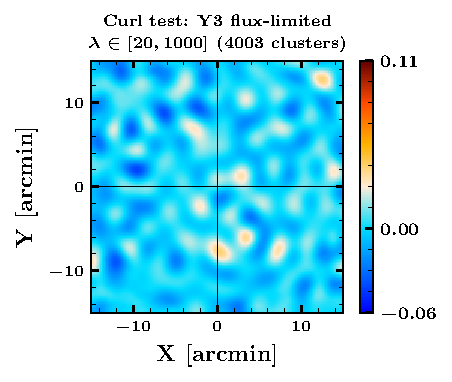
\includegraphics[width=\linewidth]{figs/kappa_model_MF_y3_v6_4_22_full_curl_test_JODY.pdf}
\caption{Stacked result of the curl test performed at the cluster locations by replacing the divergence operator in Eq. (\ref{mqe_convergence_eqn}) with a curl operator. %Both the tests are consistent with a null signal. 
We obtain a PTE value of 0.26, consistent with a null result.
%indicating that the null hypothesis of no-lensing is true.
%%The contours represent regions above $3.5\sigma$.
For the ease of visual comparison we adopt the same colour scale as in Fig. \ref{fig:fig_QE_stacked_maps}.
}
\end{figure}
\label{curl_test}
\subsection{Systematic error budget}\label{mqe_sec_systematics}

Now we quantify possible sources of systematic error. %budget for the mass constraints reported in \S\ref{sec_results}. 
%assess the robustness of the constraints on the \ML scaling relation reported in \S\ref{sec_ML_scaling} against various systematic errors. 
%The sources of systematic uncertainty we consider include
 We estimate the bias due to each cluster's SZ emission and residual foregrounds, the assumption of an underlying cluster profile, uncertainties in the DES RM mis-centering parameter $f_{\rm mis}$, approximations to the filter transfer function (Eq.~\ref{eq_filter_TF}), uncertainties in the beam measurements, and the assumption of a background cosmology.
Another source of systematic error is the uncertainties in the cluster redshifts estimated photometrically.
%But we ignore them in this work as \cite{raghunathan17a} demonstrated that the impact of photo$-z$ errors is negligible. 
However the impact of photo$-z$ errors was estimated to be negligible by \cite{raghunathan17a}, and we ignore them here.
%Throughout this section we report the bias as the shift in the average lensing mass  of the DES RM \whichyear\ flux-limited sample clusters obtained using the \ML relation with the best-fit values to be reported in Fig. \ref{fig_massrichness_fitting}.

We rely on the \cite{sehgal10} simulations to estimate the level of residual-SZ/foreground bias in the RM \whichyear{} flux-limited sample.
In all the other cases we use the data and report the shift in the average lensing mass of the clusters in the RM \whichyear{} volume-limited sample obtained in \S\ref{mqe_sec_results}. %for the \whichyear\ flux-limited sample. % with our baseline analysis \mbox{(\sptpol{} SZ-free $\times$ 150 GHz)}.
The combined systematic error budget is presented in Table~\ref{tab:sys}.
The systematic error calculated as a quadrature sum of the errors presented in Table~\ref{tab:sys} is much smaller than the statistical error in the measurements at a level of $0.15\sigma$. 
Using a direct sum, the combined error budget is $0.27\sigma$.
The dominant error comes from the uncertainty in the DES RM cluster centroids shifting the mean lensing mass by 2.8\%. 
%6.4\% for the full and volume-limited samples.

\begin{table}[ht]
\caption{Systematic error budget for DES RM volume-limited sample}
\footnotesize{
\resizebox{\columnwidth}{!}{
\centering
\begin{tabular}{| l | c | c |}
\hline
\multirow{2}{*}{Source of error} & \multicolumn{2}{c|}{Magnitude of error}\\%\hline
\cline{2-3}
& \%  & frac. of $\sigma_{stat}$ \\\hline
Beam uncertainties & $<0.01$\% & - \\\hline
Cluster mis-centering & 2.78\% & $0.12\sigma$ \\\hline
Cosmology & $0.39\%$ & $0.03\sigma$ \\\hline
Filtering $\ell_{x}$ &  0.21\% & 0.02$\sigma$\\\hline
Halo profile &  0.12\% &  0.01$\sigma$ \\\hline\hline
Residual foregrounds & 2.12\% & $0.09\sigma$\\\hline
Total & 3.53\% & 0.15$\sigma$ \\\hline
\end{tabular}
}
}
\label{tab:sys}
%\tablecomments{
%A list of systematic errors estimated for the lensing mass measurement.
%This is a list of systematic errors estimated for the lensing mass measurement.
%}
\end{table}
\subsubsection{Cluster SZ signal and residual foregrounds}\label{subsec_SZbias}

\begin{figure}
\centering

\includegraphics[width=0.45\textwidth, keepaspectratio]{figs/tSZ_bias_checks_sehgal_sims.pdf}
\caption{ Quantifying the level of bias due to residual foregrounds and the SZ signal using \citet{sehgal10} simulations. The recovered lensing mass, un-biased for the fiducial case with SZ-free map for gradient estimation and $l_{G} = 2000$ is shown as black circles. The equivalent biased results with just the 150\, GHz map and $l_{G} = 1500 (2000)$ cutoff scales for the gradient estimation are shown as red squares (orange diamonds). Each light shaded point corresponds to an individual simulation run with clusters from the DES RM Year-3 flux-limited sample. The darker data points are the values obtained for 10 $\times$ the sample size}
\label{fig_QE_sehgal_sims}
\end{figure}

In this work we eliminate the bias due to SZ signal in the reconstructed convergence maps using a SZ-free gradient map. 
%Since \sptpol{} has only two frequency channels, a simple SZ cleaning operation will tend to modify other frequency dependent foregrounds and the resultant map is not an optimal foreground free CMB map for the lensing reconstruction. 
However, projecting only the SZ signal out tends to modify other frequency-dependent foregrounds, and the resultant map is not an optimal foreground-free CMB map for the lensing reconstruction. 
This enhancement of foregrounds generally acts as an additional source of noise and tends to increase the variance of the reconstructed convergence maps. 
At the cluster locations, however, an increase in foreground emission due to galaxies inside the cluster can introduce undesired mode coupling between the SZ-free gradient map and the lensing map resulting in a biased lensing signal. 
%Since massive clusters host more galaxies, we can expect the bias to increase with the cluster mass or equivalently richness. 
Here we quantify this bias using the \cite{sehgal10} foreground simulations.

To this end, we begin with the simulated skies described in \S\ref{sims_used}, to which we then add simulated clusters, including the lensing signal (only the {\it 1-halo} term), thermal and kinetic SZ effects, and emission associated with the cluster (e.g. from member galaxies). %(like dusty galaxies). 
These simulations also include foregrounds uncorrelated with the clusters such as field radio galaxies.
The foregrounds (cluster tSZ and kSZ, radio galaxies etc.,), unless specified otherwise, come from the \cite{sehgal10} simulations described below.
%Note that the foreground maps, whether associated with the cluster or not, are not lensed by the cluster in these simulations. 
%The addition of foregrounds using \cite{sehgal10} simulations is described below. 
Note that the foreground maps, whether associated with the cluster or not, are not lensed by the cluster in these simulations. 
We expect the lensing due to foregrounds is minimal and outside the scope this thesis. 
The number of simulated clusters and their redshifts and richnesses are derived from the  DES RM \whichyear{} flux-limited sample. %check_again
The richnesses and redshifts are converted to cluster masses according to the \ML{} relation (Eq.~\ref{eq_ML}) with best-fit parameters from \citet{melchoir17}: $A_{\rm M17} = 2.35\ \times$ \munits, $\alpha_{\rm M17} = 1.12$, and $\beta_{M17} = 0.18$.  

For foregrounds, we extract half-arcminute resolution \boxsize\ cutouts of the 95 and 150 GHz \cite{sehgal10} simulations of the SZ, kSZ, radio, and infrared galaxies around halos corresponding to the mock cluster sample. %the mass and redshift of the clusters in the DES RM \whichyear\ flux-limited sample. 
We scale the SZ power down from the \cite{sehgal10} simulations by a factor of 1.75 to match the \citet{george15} measurements.
%The \cite{sehgal10} simulations contain 16,000 halos above \mvir\ $\ge$ \munits\ and 175 halos above \mvir\ $\ge 5 $ \munits\ at redshifts $z \ge 0.25$.
These foreground cutouts are added to our mock galaxy cluster lensed CMB datasets. %instead of the Gaussian realizations of the extragalactic foregrounds described earlier. 
The maps are then processed in the same way as explained in \S\ref{sec_method} to extract the SZ cleaned map and passed into the mQE. 

%Like discussed in \S\ref{sec_pipeline_validation}, we pick clusters in the richness range $\lambda \in [20, 100]$ from the DES RM \whichyear\ flux-limited sample for this test. Like in \S\ref{sec_pipeline_validation}, we use the \ML{} relation with best-fit parameters from DES \citet{melchoir17} to convert richness estimates into masses.

We present the results in Fig. \ref{fig_QE_sehgal_sims}.
%The true normalization \mbox{$A_{true} = 2.35\ \times$ \munits} adopted from \citet{melchoir17} is shown as the purple solid line.
The true normalization is shown as the purple solid line.
In the figure, the light shaded data points are the result for a single simulation run ($\sim$ 4000 clusters) and the darker data points are the results for $10\times$ the sample size. 
%As explained in \S\ref{sec_pipeline_validation}, in 
%For our baseline analysis with  maps for the gradient estimation and $\ell_{\rm G} = 2000$, the recovered normalization is $\la0.5\sigma$ from the true value.
We obtain \mbox{$A = 2.30 \pm 0.09\ \times$ \munits} (black circle) implying no significant residual foreground bias in the lensing measurements.
%This result also asserts that the lensing pipeline is unbiased.
This result also provides evidence that the lensing pipeline is unbiased.

{\it Comparison to standard QE:} We also use the \cite{sehgal10} simulations to compare the modified QE to the standard case using the 150 GHz map for the background CMB gradient estimation.
In the standard case, the correlations introduced between the two maps by the foregrounds, the SZ signal in particular, can be alleviated by lowering the LPF threshold $\ell_{\rm G}$ for the gradient map as in Eq. (\ref{mdf_eqns}). 
As described in \S\ref{sec_method}, the choice of $\ell_{\rm G}$ is a trade-off between the level of foreground bias and the lensing \snr{}. 
%Here we adopt $\ell_{\rm G} = 2000$ and $\ell_{\rm G} = 1500$.
%On the other hand, the results for the standard QE case are heavily biased: red squares (orange diamonds) for $\ell_{\rm G} = 1500$ ($\ell_{\rm G} = 2000$).
Here we adopt $\ell_{\rm G} = 2000$ and $\ell_{\rm G} = 1500$ and note that the results are heavily biased in both cases: red squares (orange diamonds) for $\ell_{\rm G} = 1500$ ($\ell_{\rm G} = 2000$).
The level of bias is higher when $\ell_{\rm G}$ is set to 2000 compared to 1500, as expected.
This bias is predominantly due to the SZ signal and can be reduced by removing massive clusters from the analysis as in \cite{baxter18}. 
For comparison, when we apply a richness cut of $\lambda \in [20, 40]$ the lensing bias is reduced from 82\% to 65\% for $\ell_{\rm G} = 2000$ and 52\% to 35\% for $\ell_{\rm G} = 1500$. 
This cut removes $\sim$500 massive clusters from the analysis.
This result can be compared to the conservative SZ-bias of 11\% set by \cite{baxter18} with $\ell_{\rm G} = 1500$ for the same richness range $\lambda \in [20, 40]$.
%They obtain a lower bias value as the high-$\ell$ modes in the SPT-SZ maps are down-weighted compared to the \sptpol{} maps which have a $4\times$ lower noise.
\cite{baxter18} obtained a lower bias value as the high-$\ell$ modes in the SPT-SZ maps are down-weighted due to $4\times$ higher noise.
%This also suggests that we cannot handle the SZ bias by simply removing clusters above a certain richness, for example $\lambda \ga 40$, for low-noise CMB datasets.

Finally, a subtle point from the figure is that the mass constraints obtained using the 150 GHz map for gradient estimation
(orange diamonds) are better ($\sim$ 14\%) than those obtained using the SZ-free map for gradient estimation (black circles) despite adopting $\ell_{\rm G} = 2000$ in both cases.
This hit in the SNR arises because the SZ-free map is noisier than the 150 GHz.
 \subsubsection{Cluster profile}\label{subsec_clusprofile}
%In our fiducial analysis we obtain lensing mass measurements by assuming that the underlying halo profile of the clusters obey the NFW dark matter model. 
%However the true profile of galaxy clusters could be different from a smooth NFW model and deviations from the NFW profile have been observed in earlier works \citep{diemer14}. 
%Furthermore, as argued by \citet{child18}, Einasto model is a better fit to `stacked' halo profiles compared to the NFW.
In our fiducial analysis, we assume that the underlying halo profile of the clusters follows the NFW dark matter model. 
However, the true profile of galaxy cluster may not follow the NFW model and indeed 
deviations from the NFW profile have been observed \citep{diemer14,child18}. %argued that the Einasto model is a better fit than NFW to stacked halo profiles.
%In this section, we estimate the bias in the lensing mass due to the assumption of the NFW profile by using an Einasto profile \citep{einasto89} to model the lensing convergence during the fitting process.
%But considering the efficacy of comparing our results to other similar works in the literature, we use NFW for our baseline analysis.

%In this section, we validate the assumption of NFW profile using an Einasto profile \citep{einasto89} to model the lensing convergence $\kappa^{1h}$ during the fitting process.
In this section, we estimate the magnitude of a possible bias due to the assumption of the incorrect mass profile by using an Einasto profile \citep{einasto89} to model the lensing convergence $\kappa^{1h}$.
% during the fitting process.
%The lensing QE and subsequently the reconstructed convergence maps remain unchanged.
The Einasto profile is defined as
\begin{eqnarray}
\rho(r)_{_{\rm Ein}} & = &  \rho_{_{0}}\ \mbox{exp}\left( - \frac{2}{\alpha} \left[\left(\frac{r}{R_{\rm s}} \right)^{\alpha} - 1\right]\right),
%\rho(r)_{_{\rm Ein}} & = &  \delta_{c}\rho_{mean}^{z}\ e^{\left( - \frac{2}{\alpha} \left[\left(\frac{r}{R_{\rm s}} \right)^{\alpha} - 1\right]\right)}
\label{eq_einasto_density}
\end{eqnarray}\\
%where $R_{\rm s}$ is the scale radius, $\delta_{c}$ is the characteristic over-density, $\rho_{mean}^{z}$ is the mean-density of the Universe at the cluster redshift, and $\alpha = 0.18$ is the shape parameter \citep{ludlow13}. 
where $\alpha = 0.18$ is the shape parameter \citep{ludlow13}. 
As in the NFW analysis, the concentration $c_{200}$ as a function of mass and cluster redshift is obtained using the \citet{duffy08} relation.
We use the general framework for spherically symmetric halos defined in the previous chapter \ref{ch:MLE} and simply plug the above density profile into Eq. \ref{eq:sr_den} to obtain the Einasto convergence \kappaonehalo$^{,\rm Ein}$ profiles. The \kappatwohalo\ term remains the same. For the Einasto case we see a negligible shift of $0.01\sigma$ compared to our fiducial result.
%The shift in the lensing mass of the DES RM clusters is negligible. 
\subsubsection{Uncertainties in filter transfer function and beam}\label{subsec_TF}
As described in \S\ref{sec_data}, the \sptpol{} map-making process is lossy, with noisy modes along the scan direction filtered out. 
The ideal, if computationally expensive, approach to handle the filtering would be an end-to-end simulation from the TOD to the lensing reconstruction. 
In this work, we take a computationally much cheaper approach and approximate the filtering by the phenomenological fit to the filter transfer function in Fourier space given by Eq. (\ref{eq_filter_TF}). 
The major uncertainty is in the position of the high-pass filter (HPF) in the scan direction: this filters modes more strongly than the isotropic HPF, and the LPF is at angular scales that do not matter to the reconstruction. 
The estimated position for this HPF is $\ell_x = 300 \pm 20$. 
%Thus we evaluate the recovered mass for an assumed $\ell_x=$280 and 320 in Eq. \ref{eq_filter_TF}.
%The model, however, remains fixed at $\ell_x = 300$ in both the cases.
We also recompute the models for an assumed $\ell_x = 280$ and 320 to evaluate the shifts in the lensing masses.
%Ideally, one can expect the lensing masses to shift low and high for the two cases compared to our fiducial result.
We note no significant effect (masses shift by roughly $\pm 0.02\sigma$), indicating that the uncertainty in the simplified filtering treatment causes negligible changes to our results.
%%\pending{Pending: SR: Will it be better to test this using simulations instead?.}

Similarly, we also check the effect of errors in the telescope beam modeling \beambl{} that were derived using Venus observations (see \S\ref{sec_sptpol}). 
We find that the effect due to beam uncertainties in the final result is also negligible. 
The shift in the lensing mass is $\le 0.01\sigma$ when we modify \beambl{} $\rightarrow$ \beambl{} $+\ 2\sigma$.
%For the Einasto profile we obtain a lensing mass of \sysbiaseinastoresult\ for the stacked sample. While the mass is slightly higher, it is only $0.2\sigma$ off from our fiducial result implying that the bias due to the assumption of the NFW profile is negligible. 
\subsubsection{Underlying cosmology}\label{subsec_others}
%In this section we estimate the effect of the assumption of a background cosmology on the lensing measurements. 
The systematic error arising due to the assumption of a background cosmology is quantified here.
As described in earlier sections, in our fiducial analysis we use the $\Lambda$CDM cosmology obtained using the \citet{planck15-13} datasets. 
%Here we repeat the analysis by slightly changing the background cosmology. 
%Specifically, we generate new lensed CMB power spectra using \texttt{CAMB} by adding $1\sigma$ errors to the \planck\ 2015 cosmological parameters and similarly by altering the beam by \beambl $+\ 2\sigma$. 
Here we repeat the analysis by modifying the lensed CMB power spectra $C_{\ell}$ to include the $1\sigma$ errors to the  \citet{planck15-13} cosmological parameters.
Modifying the background cosmology alters the weights of Eq. (\ref{mdf_eqns}) in the lensing estimator and also the model convergence profiles \kappaonehalomz\ and \kappatwohalomz. 
However, the effect due to background cosmology in the inferred lensing mass is negligible with a shift in the lensing mass $\le 0.03\sigma$.
%\subsection{Offsets in the stacked convergence map}\label{subsec_offsets}
%\section{NFW profile}
\subsubsection{Uncertainties in $f_{\rm mis}$ parameter}\label{subsec_mis-centering}
In our baseline analysis we perform a mis-centering correction of the cluster convergence models (see \S\ref{sec_model_fitting}) using $f_{\rm mis} = 0.22$ based on the results by \citet{rykoff16} for the RM clusters from the science verification data.
%In this section 
Now we generate new convergence models assuming a larger fraction, 33\%, of the clusters are mis-centered by modifying the mis-centering parameter by its $1\sigma$ error 
%($f_{\rm mis} = 0.33$) 
from \citet{rykoff16}. %and check the effect on the inferred lensing masses. % obtained in this work.
Since the two parameters, $f_{\rm mis}$ and $c_{\rm mis}$, describing the cluster mis-centering are highly correlated, we also modify \mbox{ln $c_{\rm mis}$} = -1.32 for this test. 

The recovered mass increases by 2.8\% in this case.
However, the shift is only $0.12\sigma$, $1/8^{th}$ of the statistical uncertainty. % well within the statistical uncertainty and $\sim0.3\sigma$ of the original result.
The direction of the shift is consistent with expectations, as assuming a larger $f_{\rm mis}$ should smear the convergence model more than the fiducial case leading to an increased lensing mass. 
Since this is the dominant systematic, we also estimate the error for the flux-limited sample.
The mean lensing mass of the volume-limited sample goes up 3.2\% but the change is still smaller than the statistical error ($0.16\sigma$). 
  \section{Results and Discussion}\label{mqe_sec_results}

The main results of this work are the lensing-derived cluster mass constraints for the DES RM \whichyear\ cluster samples using \sptpol{} SZ-free gradient maps $\times$ 150 GHz temperature maps.
%using three different combination of the \sptpol{} and \planck{} temperature maps: (A) \sptpol{} SZ-free $\times$ 150 GHz maps (baseline); (B) \lgmca $\times$ \sptpol 150 GHz maps; and (C) baseline $+$ \sptpol{} SZ-free $\times$ SZ-free maps for clusters with $\lambda \ga 40$.
Below, we first present the lensing mass estimates in \S\ref{sec_temp_results} and use the lensing measurements from the DES \whichyear{} volume-limited sample to independently calibrate the \ML{} relation of the cluster sample in \S\ref{sec_ML_scaling}. 
\subsection{Stacked mass measurements}
\label{sec_temp_results}
In Fig. \ref{fig:fig_QE_stacked_maps}, we present the results of our stacked lensing measurements. 
The left (right) panel correspond to the convergence maps stacked at the location of clusters in the DES \whichyear\ flux(volume)-limited sample.
The variance in the flux-limited sample is lower than the volume-limited sample because the flux-limited sample has twice as many objects. 
An estimate of the mean-field has been subtracted from the maps.
We reject the null hypothesis of no lensing with a significance of \howmanysigmaforfullsample\ for the flux-limited sample of \howmanyclustersinfullsample\ clusters. 
The obtained \snr{} is consistent with our expectations from the simulations shown as lighter black circles in Fig. \ref{fig_QE_sehgal_sims}.
For the smaller volume-limited sample, the no-lensing hypothesis is ruled out at  \howmanysigmaforcosmosample.
The radially binned convergence profiles that are used to estimate the cluster masses are shown in Fig. \ref{fig:avg_fig_QE_stacked_maps} along with the best-fit model curves. 
\begin{figure}
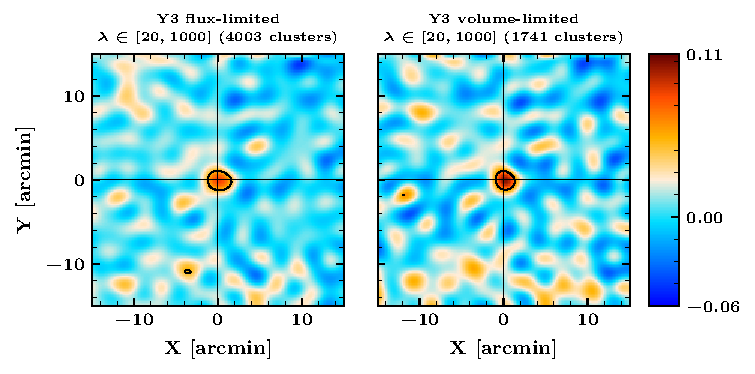
\includegraphics[width=\linewidth]{figs/kappa_model_MF_y3_v6_4_22_full_vl_JODY.pdf}
\caption{The inverse-variance weighted stacked convergence maps at the location of 4002 and 1741 clusters in the range $\lambda$ $\in$ [20,1000] from flux limited (left) and the volume-limited (right) samples of the DES RM Year-3 cluster catalog. The contour corresponds to the regions above $3.5 \sigma$. The null hypothesis of no-lensing is rejected at $8.7\sigma$ and $6.7 \sigma $ for the two cases respectively.}
\label{fig:fig_QE_stacked_maps}
\end{figure}

\begin{figure}[ht]
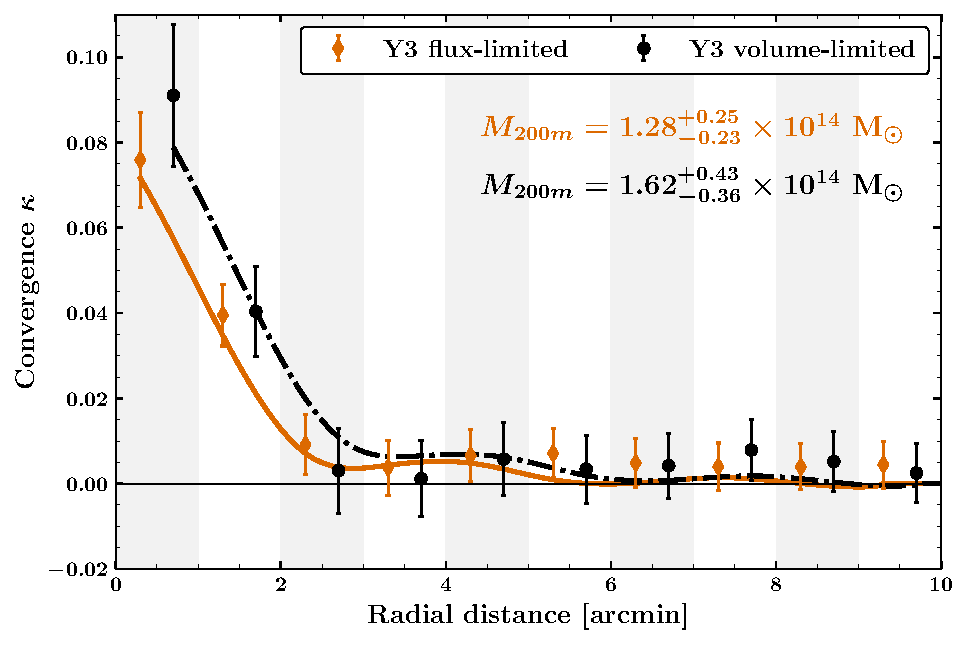
\includegraphics[width=\linewidth]{figs/kappa_model_MF_y3_v6_4_22_full_vl_radprf_JODY.pdf}
\caption{The azimuthally averaged radial profile of the stacked convergence maps from Fig. ~\ref{fig:fig_QE_stacked_maps}. The black circles and orange diamonds correspond to the flux and volume-limited Year-3 DES RM cluster samples. The error bars are the diagonal value of the covariance matrix estimated using the jackknife technique in Eq. ~\ref{eq_JK_cov}. The data points for the two samples have been artificially shifted from the bin centres to avoid cluttering (orange diamonds are shifted to left and solid black circles to right). }
\label{fig:avg_fig_QE_stacked_maps}
\end{figure}

The ringing pattern is because of the sharp filtering of modes above the \sptpol{} beam scale. 
The error bars plotted are the square root of the diagonal entries of the covariance matrix estimated using Eq. (\ref{eq_JK_cov}). 
%As explained in \S\ref{sec_nfw_model_fitting}, all the mass estimates are derived by fitting a NFW profile along with the contribution from the {\it 2-halo} term to the measured radially binned profile. 
The recovered lensing masses for the stacked flux and volume-limited samples are $M_{200m} = 1.28^{+0.14}_{-0.18} \times 10^{14} M_{\odot}$ and $1.62^{+0.32}_{-0.25} \times 10^{14} M_{\odot}$ respectively. %\mbox{\mvir = \fitmassforfullsamplewitherrors\ \times \munits} and \mbox{\fitmassforvlsamplewitherrors\ \times \munits} respectively. 
According to expectations, the lensing masses shift up by 0.3$\sigma$ when the {\it 2-halo} term is excluded.


A higher mean mass is expected for the volume-limited sample. 
At redshifts above $z\sim 0.6$, galaxies at the luminosity threshold adopted by RM become too faint to be detected in the DES data. 
Consequently, the richness of the clusters is extrapolated from the subset of galaxies that are sufficiently bright to be detected. 
This extrapolation introduces additional noise in the richness estimates.
The increased scatter leads to more low-mass systems scattering up to apparently rich systems, thereby lowering the mean mass of the selected halos. 
For this reason, we restrict our analysis to the volume-limited sample in the subsequent sections. 
\subsection{Mass-richness \ML{} scaling relation calibration}\label{sec_ML_scaling}

We now apply the lensing mass measurements from \S\ref{sec_temp_results} to constrain the relationship between a cluster's mass, $M$, and optical richness, $\lambda$, in the DES RM \whichyear{} volume-limited sample. 
We limit the analysis to just the volume-limited sample since the flux-limited sample has selection bias as explained previously in \S\ref{sec_temp_results}.
%Due to its higher S/N, we use the QE  with a SZ-free gradient map; we do not combine the two estimators due to the complexity in combining the different bases of the MLE and QE. 
Following earlier weak-lensing analyses of RM clusters \citep{simet18, melchoir17, mcclintock18}, we use a power-law scaling relation for cluster mass, $M$, as a function of richness, $\lambda$, and redshift, $z$,
\begin{eqnarray}
M = A \left(\frac{\lambda}{40}\right)^{\alpha} \left(\frac{1+z}{1+0.35}\right)^{\beta},
\label{eq_ML}
 \end{eqnarray}
 where $A$ is a normalization parameter, and the exponents $\alpha$ and $\beta$ are richness and redshift evolution parameters respectively. 
The pivot points for the richness and redshift evolution parameters were set based on DES weak-lensing measurements of \cite{mcclintock18}.
%Given the total\snr{}is of order eight for the flux-limited sample, we do not subdivide the stacks into different richness or redshift bins. 
The model for the stacked mass is 
\begin{equation}
M(A, \alpha, \beta) \equiv M = \frac{\sum_j w_j M(\lambda_{j}, z_{j})}{\sum_j w_j}, 
\label{eq_model_ML}
\end{equation}
where the sum runs over the number of clusters in the sample and the weight $w$ for each cluster is given in Eq. (\ref{eq_cluster_weight}).
\begin{figure}[ht]
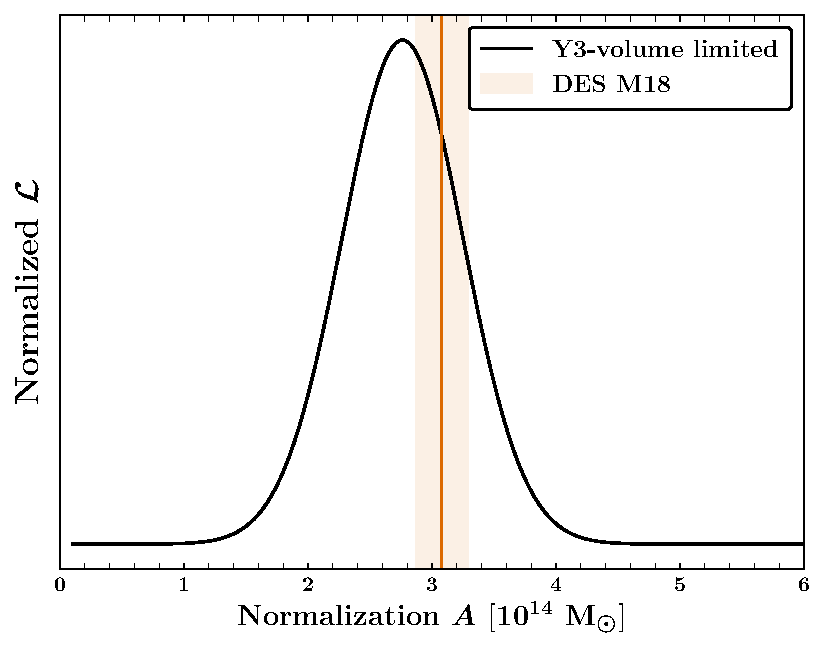
\includegraphics[width=\linewidth]{figs/M_rich_fitting_y3_v6_4_22_full_vl_JODY.pdf}
\caption{Marginalized posteriors of the normalization parameter A of the M-$\lambda$ relation for the volume-limited sample of the RM cluster-catalog. The result is consistent with the best-fit values obtained by DES weak-lensing measurements \citet{mcclintock18}, shown as the shaded region}
\label{fig_massrichness_fitting}
\end{figure}

We do not split the stacks into different richness or redshift bins.
As a result, the data's sensitivity to the two evolution parameters is minimal and we apply informative priors to both.
We perform a Markov chain Monte Carlo (MCMC) analysis %with 100 walkers and 750 steps each 
using the publicly available \emph{emcee} \citep{mackey13} code to sample the likelihood space.
We assume a flat prior for the normalization parameter $A$ in the range $A \in [0.1,100]\ \times$ \munits. 
For the slopes, we use a Gaussian prior based on \citet{mcclintock18}. Specifically, we set $(\alpha_{0}, \sigma_{\alpha})= (1.356, 0.056)$ and $(\beta_{0}, \sigma_{\beta})= (-0.3, 0.3)$. 
The posteriors on both the richness evolution parameters, as expected, follow the assumed prior. % and are hence not shown. 
We obtain a normalization value of $A = 2.70^{+0.51}_{-0.50} \times 10^{14} M_{\odot}$, which is consistent with results from DES weak-lensing measurements of $A_{\rm DES} = 3.08 \pm 0.21 \times$ \munits{} by \citet{mcclintock18}. 
The marginizalized posterior for $A$ is shown as the black curve in Fig. \ref{fig_massrichness_fitting} along with measurements from \citet{mcclintock18} as the orange shaded region.
%The first 100 steps from all walkers were discarded as the burn-in phase.

\iffalse{
\begin{figure}[ht]
\centering
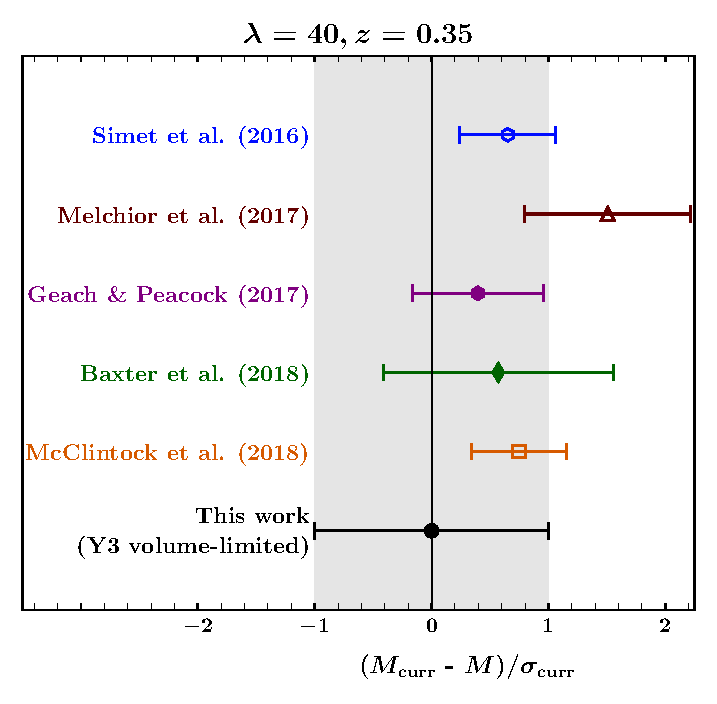
\includegraphics{figs/lit_comparisons_JODY.pdf}
\caption{Comparison of $M_{200m}$ mass estimates of galaxy clusters obtained using the M-$\lambda$ relation from different works in the literature using the RM cluster catalogs. The points have been normalized using the $1\sigma$ error from the analysis with the Year-3 volume-limited sample of the DES RM catalog. The filled (open) points represent measurements using the CMB-cluster lensing (galaxy weak-lensing) technique}
\label{fig_lit_comparison}
\end{figure}
\subsection{Comparison to literature}\label{subsec_lit_comparison}
We now compare our results to similar works from the literature performed with the RM cluster catalogs from the SDSS and DES experiments. 
Since the richness estimated for a given cluster from surveys A and B can vary slightly depending on the adopted data reduction and analysis choices, we include a small correction factor $\epsilon_{\rm A{\text -}B}$ when comparing results from two surveys.
We compute the ratio $\lambda_{\rm A}/\lambda_{\rm B}$ for the overlapping clusters in the two surveys and simply set $\epsilon_{\rm A{\text -}B}$ to the median value of the ratios.
We find the richness estimates in DES Year-3 and Year-1 to be consistent with $\epsilon_{\rm Y3{\text -}Y1} = 1$. 
For the rest, we set: $\epsilon_{\rm Y3{\text -}SV} = 1.08$ and $\epsilon_{\rm Y3{\text -}SDSS} = 0.93$ \cite{mcclintock18}.
The comparison after including this correction factor is presented in Fig. \ref{fig_lit_comparison}, which is similar to Fig. 15 in \cite{mcclintock18}. 
%Specifically, we show the difference in \mvir masses obtained from different works for a cluster with richness $\lambda = 40$ at redshift $z=0.35$, the pivot points in Eq. (\ref{eq_ML}).
The figure is normalized using the $1\sigma$ error from the current work with the \whichyear{} volume-limited DES RM catalog sample.

%In the figure, \citet{simet18} and \citet{geach17} works use the SDSS RM catalog sample containing roughly 26,000 clusters while the other use DES RM catalogs.
Each analysis uses a different cluster sample and lensing data.
\citet{simet18} and \citet{geach17} use the SDSS RM catalog sample containing roughly 26,000 clusters. % while the other use DES RM catalogs.
%Among the DES works, 
\citet{melchoir17} use the full catalog from the DES science verification data while \cite{baxter18} and \cite{mcclintock18} perform the analysis using the DES Year-1 volume-limited sample.
The works by \citet{geach17} and \cite{baxter18} use the CMB-cluster lensing technique (filled points) with \planck{} and {\sc SPT-SZ} CMB temperature maps.
All the others use galaxy weak-lensing measurements and are represented as open points. As evident from the figure, our results are consistent with other similar works in the literature.
}\fi
\section{Conclusions}
\label{sec_con}

In this chapter, we introduced the quadratic estimator which extracts CMB-cluster lensing signal by exploiting the correlation between the gradient map and lensing map. 
Though QE is just a first order approximation, it holds excellently well even in the strong lensing regime as CMB doesn't have structures at galaxy cluster angular scales. 
The SZ effect acts as a major source of systematic and statistical contaminant for CMB-cluster lensing analysis.
We developed a modified QE to eliminate the SZ induced systematic bias. 
In the modified QE, the undesired SZ correlation between the gradient and the lensing map can be eliminated by using an SZ-free gradient map with only a slight decrease of SNR. 
%We modified the QE to eliminate the SZ bias with negligible affect on the SNR.
Our pipeline returned unbiased results when tested using simulations. 
 
We used our proposed method to constrain the mass of DES year-3 cluster catalog.
The DES year-3 catalog consists of 4002 (1741) clusters in the full (volume) limited sample. 
We model the lensing convergence profile assuming a NFW profile and found the average mass of full (volume) limited cluster sample to be $M_{200m} = 1.28^{+0.14}_{-0.18}$ ($M_{200m} = 1.62^{+0.32}_{-0.25}$). 
In addition to that, we also reported several sources of systematics in Table \ref{tab:sys} and found that all the systematics are much smaller than the statistical error.% cluster centroids to be dominant systematic source. 



  
 
